%% PNAStwoS.tex
%% Sample file to use for PNAS articles prepared in LaTeX
%% For two column PNAS articles
%% Version: Apr 15, 2008


%% BASIC CLASS FILE
%\documentclass{pnastwo}
\documentclass[11pt]{article}
\usepackage[hang,flushmargin]{footmisc}
\usepackage{mathtools}
\usepackage{capt-of}
\usepackage{xcolor}
%% ADDITIONAL OPTIONAL STYLE FILES
\usepackage{mathptmx}
\usepackage{graphicx}
\usepackage[margin=1in]{geometry}
%\newcommand{\rom}[1]{\uppercase\expandafter{\romannumeral #1\relax}}%\usepackage{titlesec}
%\usepackage[pdftex]{graphicx}
%\usepactxkage{pnastwoF}
\usepackage{amssymb,amsfonts,amsmath}
%\usepackage[numbers,sort&compress]{natbib}
\usepackage{mhchem}
%\usepackage{subeqnarray}
%\usepackage{cases}
\usepackage{color}
\usepackage{verbatim}
\usepackage{xcolor}
%\usepackage{romannum}
\usepackage{braket}
\usepackage{siunitx}
\usepackage{tocloft}
\usepackage{units}
\usepackage{array}
\usepackage{longtable}
\usepackage{tabularx}
\usepackage{multirow}
\usepackage[skins,theorems]{tcolorbox}
\tcbset{highlight math style={enhanced,
  colframe=red,colback=white,arc=0pt,boxrule=1pt}}
\renewcommand\thesection{\arabic{section}}
%\usepackage[figurename=Figure.,
%                  justification=RaggedRight,
%                  labelfont={bf, footnotesize},
%                  textfont={footnotesize},position=top]{caption}
\usepackage{array}
\usepackage{longtable}
\usepackage{tabularx}
\usepackage{multirow}
\usepackage{fixltx2e}
\usepackage{textgreek}
\usepackage[T1]{fontenc}
%\usepackage{ulem}
\usepackage[normalem]{ulem} %to strike the words
\newcolumntype{C}[1]{>{\arraybackslash}p{#1}}
\usepackage[labelfont=bf]{caption}


\usepackage{color} %for \textcolor
\usepackage{epsfig}
\usepackage{floatflt}
\usepackage{wrapfig}
%\usepackage{titlesec}


\usepackage{float}
\usepackage{times}
\usepackage{helvet}
\usepackage{amsmath}
\headheight = 0.0 in
\headsep = 0.0 in

\newcommand{\todo}[1]{{\color{red}{[#1]}}}
\renewcommand{\thefootnote}{\fnsymbol{footnote}}
%\renewcommand{\thesection}{\Alph{section}}
\renewcommand{\familydefault}{\sfdefault}

\setcounter{secnumdepth}{5}
\setcounter{tocdepth}{5}


\long\def\symbolfootnote[#1]#2{\begingroup%
\def\thefootnote{\fnsymbol{footnote}}\footnote[#1]{#2}\endgroup}

\renewcommand{\figurename}{{Fig.}}

\newcommand{\ra}{\rightarrow}
\newcommand{\nubot}{nubot}
\newcommand{\degree}{$^{\circ}$C}

\long\def\remove #1{}

\newcommand{\red}[1]{\textcolor{red}{#1}}
\newcommand{\redd}[1]{\textcolor{red}{#1}}
\newcommand{\peng}[1]{\textcolor{red}{peng: #1}}
\newcommand{\tbd}[1]{\textcolor{red}{To be added: #1}}


%\setcounter{page}{1} \pagenumbering{arabic}
\pagestyle{plain} \setcounter{page}{1} \pagenumbering{arabic}

%\renewcommand{\theequation}{S\arabic{equation}}
%\renewcommand{\figurename}{\textbf{Supplemental Figure}}
%\renewcommand{\tablename}{\textbf{Supplemental Table}}
%\renewcommand{\thefigure}{S\arabic{figure}}
%\renewcommand{\thetable}{S\arabic{table}}
%\usepackage{helvet}
\renewcommand{\familydefault}{\sfdefault}
%\usepackage[T1]{fontenc}
%\usepackage{fourier}
%\usepackage{cmbright}
%\usepackage{etoolbox}
%\patchcmd{\thebibliography}{\section*{\refname}}{}{}{}
\renewcommand\refname{}
%\textcolor{black}{}
%\newcommand{\blackt}[1]{\textcolor{black}{#1}}
%\newcommand{\blue}[1]{\textcolor{red}{#1}}
\newcommand{\sub}[1]{\textsubscript{#1}}
\newcommand{\supp}[1]{\textsuperscript{#1}}
\renewcommand{\thefootnote}{$\dagger$}
\newcommand{\redt}[1]{\textcolor{black}{#1}}
\newcommand{\aeb}[1]{\textcolor{black}{#1}}
\newcommand{\aebN}[1]{\textcolor{black}{#1}}
\newcommand{\orangecl}[1]{\textcolor{black}{#1}}
\newcommand{\clred}[1]{\textcolor{red}{#1}}
\newcommand{\clblue}[1]{\textcolor{blue}{#1}}
\newcommand{\clredd}[1]{\textcolor{black}{#1}}
\newcommand{\clredtable}[1]{\color{black}{#1}}
\newcommand{\tsub}[1]{\textsubscript{#1}}
\newcommand{\tsup}[1]{\textsuperscript{#1}}
 \renewcommand{\familydefault}{\sfdefault}

\DeclareSIUnit{\molar}{M}
\DeclareSIUnit{\nucl}{nucl.}
\DeclareSIUnit{\aa}{aa}

%\newcommand{\supp}[1]{\supp{#1}}
%\usepackage{mathpazo}
%% OPTIONAL MACRO DEFINITIONS
%\def\s{\sigma}
\usepackage[
singlelinecheck=true % <-- important
]{caption}

\makeatletter
\renewcommand\paragraph{\@startsection{paragraph}{4}{\z@}%
            {-2.5ex\@plus -1ex \@minus -.25ex}%
            {1.25ex \@plus .25ex}%
            {\small\small\bfseries}}
\makeatother
\setcounter{secnumdepth}{4} % how many sectioning levels to assign numbers to
\setcounter{tocdepth}{4}    % how many sectioning levels to show in ToC
%\usepackage[sort, numbers]{natbib}
%\setcitestyle{square}
%\setcounter{secnumdepth}{4}

%\titleformat{\paragraph}
%{\normalfont\normalsize\bfseries}{\theparagraph}{1em}{}
%\titlespacing*{\paragraph}
%{0pt}{3.25ex plus 1ex minus .2ex}{1.5ex plus .2ex}

\renewcommand{\contentsname}{}
\renewcommand*\subsectionmark[1]{\markright{#1}}
\renewcommand{\thesubsection}{\arabic{subsection}}


\begin{document}

\title{Integrative Modeling of Bacterial H2O2 Stress Responses}
\author{Chen Liao}

\maketitle
\tableofcontents

%\begin{abstract}
%The abstract text goes here.
%\end{abstract}

\section{Background knowledge}

Reactive oxygen species (ROS) such as superoxide, hydrogen peroxide (H2O2), and hydroxyl radical, can be produced by intracellular aerobic respiration and/or environments. They are toxic to bacterial cells, leading to loss of fitness, including high mutation rates, growth defects, and even cell death. Biochemically, there are two basic classes of H2O2-degrading proteins
\begin{enumerate}
\centering
\item{Catalase: $2H_2O_2 \rightarrow O_2+2H_2O$}
\item{Peroxidases: $RH_2+H_2O_2 \rightarrow R+2H_2O$}
\end{enumerate}
The electron source of catalase is from H2O2 itself and no exogenous electron source is needed. However, peroxidases can differ in their electron donors (i.e., $RH_2$), which could be glutathione, thioredoxins, NAD(P)H, cytochrome \textit{c}, dyes and other unknowns. 

Catalases rely on iron or manganese so they fall into two categories: heme (an iron-containing compound) calatases and non-heme catalases (or manganese). Catalases with only catalatic activity are called mono-functional catalases, and those with both catalatic activity and peroxidatic activities are referred to as bifunctional catalases or catalase-peroxidases. The activity of catalase-peroxidases is low (ca. 1\% of the maximum catalase activity) and thus seems unlikely to be an important contributor to H2O2 degradation.

Peroxidases also fall into two categories: thiol (i.e., RSH)-based peroxidases (peroxiredoxins; abbr. Prx) and non-thiol peroxidases. All peroxiredoxins contain a conserved cysteine that reacts with H2O2 and forms a disulfiide before getting reduced back to free thiol. Depending on the variations in the mechanisms of thiol regeneration, peroxidases can be further calssfied into four groups: alkylhydroperoxide reductases (AhpCF), thiol glutathione peroxidase (Tpx), bacterioferritin comigratory protein (BCP), and glutathione peroxidase (Gpx). 

\subsection{\textit{Escherichia coli}}

Most of the following information about \textit{E. coli} antioxidant systems come from a review paper~\cite{mishra2012bacteria}. \textit{E. coli} has at least 9 enzymes that have been proposed to be calatases or peroxidases. The major H2O2 scavenging enzyme is Ahp (alkyl hydroperoxide reductase)~\cite{seaver2001alkyl}, which consists of two subunits: the small subunit (AhpC), which reduces organic peroxides to their corresponding alcohols, and the large subunit (AhpF), which is involved in the regeneration of oxidized AhpC. AhpF needs NAD(P)H as an electron donor: electron movement within AhpF occurs from NAD(P)H to FAD, from FAD to a C345/C348 thiol/disulfide center, and from thiols to the N-terminal redox-active center (C129/C132). Therefore, Ahp has limited activity under conditions when reducing power is limited (e.g., nutrient starvation).

In the meanwhile, \textit{E. coli} contains two catalases, HPI (hydroperoxidase I, encoded by \textit{katG}) and HPII (hydroperoxidase II, encoded by \textit{katE}). Despite the key role of Ahp, catalase still has an important role in wild-type cells, because the activity of Ahp is saturated at a low concentration of H2O2. In contrast, catalase has a high Km, and it therefore becomes the predominant scavenger when H2O2 concentrations are high. In addition, catalases provide protection even in energy-depleted cells.

When the entry rate of H2O2 is high, basal level defense is inadequate and adaptive response is needed. HPI is transcriptionally induced during the lag~\cite{madar2013promoter}/log phase in response to low concentrations of H2O2 and this induction requires the transcriptional regulator, OxyR, which also induces \textit{ahpC}. A key cysteine residue of the OxyR protein is oxidized by H2O2, triggering conformational change from an inactive form (i.e., reduced state) to an active form (oxidized state). The oxidized OxyR then binds to the promoter regions of many genes on the \textit{oxyR} regulon. OxyR positively controls genes for peroxide detoxification, such as catalase and peroxiredoxin (katG, ahpCF), Fe-storage miniferritin (dps), glutaredoxin, thioredoxin and glutathione reductase (grxA, trxC, gor), sulfenic acid oxidoreductase (dsbG), ferric uptake regulator (fur), Fe-S-cluster assembly machinery (sufABCDE), ferrochelatase (hemH), manganese import (mntH) and the small RNA (oxyS)~\cite{hillion2015thiol}. OxyR negatively regulates its own expression and that of the genes for the ferric ion reductase (fhuF), the outer membrane protein (flu), the mannonate hydrolase (uxuAB) and gluconate permease (gntP)~\cite{hillion2015thiol}. OxyR is regenerated by the glutaredoxin/GSH/Gor system upon return to non-stress conditions. In contrast to HPI and Ahp, HPII is induced at the transition from exponential phase to stationary phase by RpoS and its induction is OxyR-independent. Mutatino in HPII did not affect the log-phase growth phenotype even in strains lacking HPI and/or Ahp~\cite{seaver2001alkyl}.

Other peroxidases seem to play other functions than H2O2-degradation \textit{in vivo}, although their activity has been demonstrated. For example, the \textit{tpx} mutant did not show any phenotype under aerobic growth, while it is more sensitive to organic hydroperoxides. Deletion of \textit{btuE} (Gpx) also does not create sensitivity to H2O2, while the mutant is more sensitive to paraquat and tellurite. In addition, the \textit{E. coli} btuE gene is not induced during H2O2 stress and overexpressing of this gene does not confer protection for cells lacking other antioxidant enzymes.

\subsection{\textit{Pseudomonas aeruginosa}}

KatA is the major catalase in \textit{P. aeruginosa} whose expression is constitutively highly in all phases of growth (high basal) but increased upon stationary growth phase and H2O2 treatment~\cite{heo2010major}. It is highly stable and can be found in the extracellular milieu, which ensures the survival of \textit{P. aeruginosa} cells in its biofilm state. Other typical antioxidant enzymes for the defense against H2O2 challenges include catalases (KatB and KatE) andalkyl hydroperoxide-reducing proteins (AhpB, AhpC, and Ohr). The \textit{katA}, \textit{katB}, \textit{ahpB}, and \textit{ahpCF} genes are positively regulated by OxyR in response to H2O2 and menadione or paraquat (PQ) treatments. KatA was also found to be regulated by quorum sensing signals~\cite{hassett1999quorum}. Recently, it was reported that KatE was induced by high temperature and requires the disulfide bond formation system for its activity.

It was also found that inactivation of the \textit{P. aeruginosa} stringent response (SR), a starvation stress response controlled by the alarmone (p)ppGpp, caused impaired antioxidant defenses and antibiotic tolerance. Upon amino acid starvation, induction of the SR upregulated catalase activity. Full expression of \textit{katA} and \textit{katB} also required the SR, and this regulation occurred through both RpoS-independent and RpoS-dependent mechanisms. Overexpression of \textit{katA} was sufficient to restore H2O2 tolerance and to partially rescue the antibiotic tolerance of SR cells.

%%%%%%%%%%%%%%%%%%%%
%%%%%%%%%%%%%%%%%%%%
%%%%%%%%%%%%%%%%%%%%
\section{Modeling H2O2 diffusion, production and decomposition}

Fig.~\ref{fig:h2o2_decomposition_schematic_diagram} shows the schematic diagram of H2O2 diffusion, production and decomposition.

\begin{figure}[h!]
\centering
  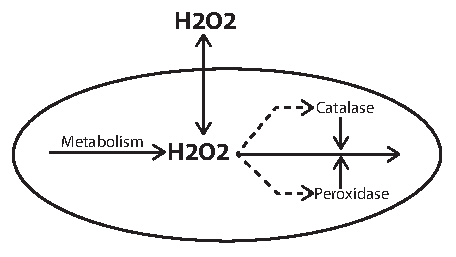
\includegraphics[width=0.5\linewidth]{h2o2_decomposition.pdf}
  \caption{Schematic diagram of H2O2 reactions.}
  \label{fig:h2o2_decomposition_schematic_diagram}
\end{figure}

%%%%%%%%%%%%%%%%%%%%
\subsection{Unregulated model (constant Ahp and KatG)}
\clblue{We assume that extracellular H2O2 ($[H_{o}]$) is a constant and intracellular H2O2 ($[H_{i}]$) is produced at a constant rate. Two enzymes, Ahp and KatG, are considered but their enzyme concentrations are assumed constant as well.} In \textit{E. coli}, Ahp becomes saturated at a low concentration of H2O2 (low $K_m$), while catalase has a high $K_m$. Therefore, decomposition of H2O2 by Ahp and catalase are modelled using Michaelis-Menten and first-order equation respectively. The model for intracellular H2O2 at steady state is
\begin{equation}
\frac{dH_i}{dt} = k_{met}+([H_o]-[H_i])PA - k_{cat}[H_i] - \frac{k_{ahp}[H_i]}{K_{m,ahp}+[H_i]}
\end{equation}
where the four terms represent intracellular production rate ($k_{met}$), diffusion based exchange, decomposition by catalase and decomposition by Ahp respectively. $P$ is permeability coefficient and $A$ is the surface area of the membrane. $k_{cat}$ and $k_{ahp}$ are the maximum decomposition rates by catalase and Ahp respectively. At steady state, we can solve $[H_i]$ as a function of $[H_o]$
\begin{eqnarray}
[H_i] &=& \frac{-\Delta +\sqrt{\Delta^2+4K_{m,ahp}(PA+k_{cat})(k_{met}+[H_o]PA)}}{2(PA+k_{cat})}  \label{eq:hi_ho}\\
\Delta &=& K_{m,ahp}PA+K_{m,ahp}k_{cat}-[H_o]PA-k_{met}+k_{ahp}
\end{eqnarray}
The following parameter values are collected from Seaver and Imlay~\cite{seaver2001hydrogen} for \textit{E. coli} cells: $P=1.6\times 10^{-3}~cm/s$, $A=1.41\times  10^{-7}~cm^2$, $k_{met}=4.5\times 10^{-20}~mol/s$, $k_{cat}=2.7\times 10^{-13}~L/s$, $k_{ahp}=2.1\times 10^{-18}~mol/s$, $K_{m,ahp} = 1.2\times 10^{-6}~M$. See Fig.~\ref{fig:rHoHi} for simulated $[H_o]/[H_i]$ ratio for wild-type cell, Catalase mutant, Ahp mutant, and double mutant. Using this set of parameters, the intracellular H2O2 concentration can be as low as 10 fold less to the extracelluar concentration of H2O2.

\begin{figure}[h!]
\centering
  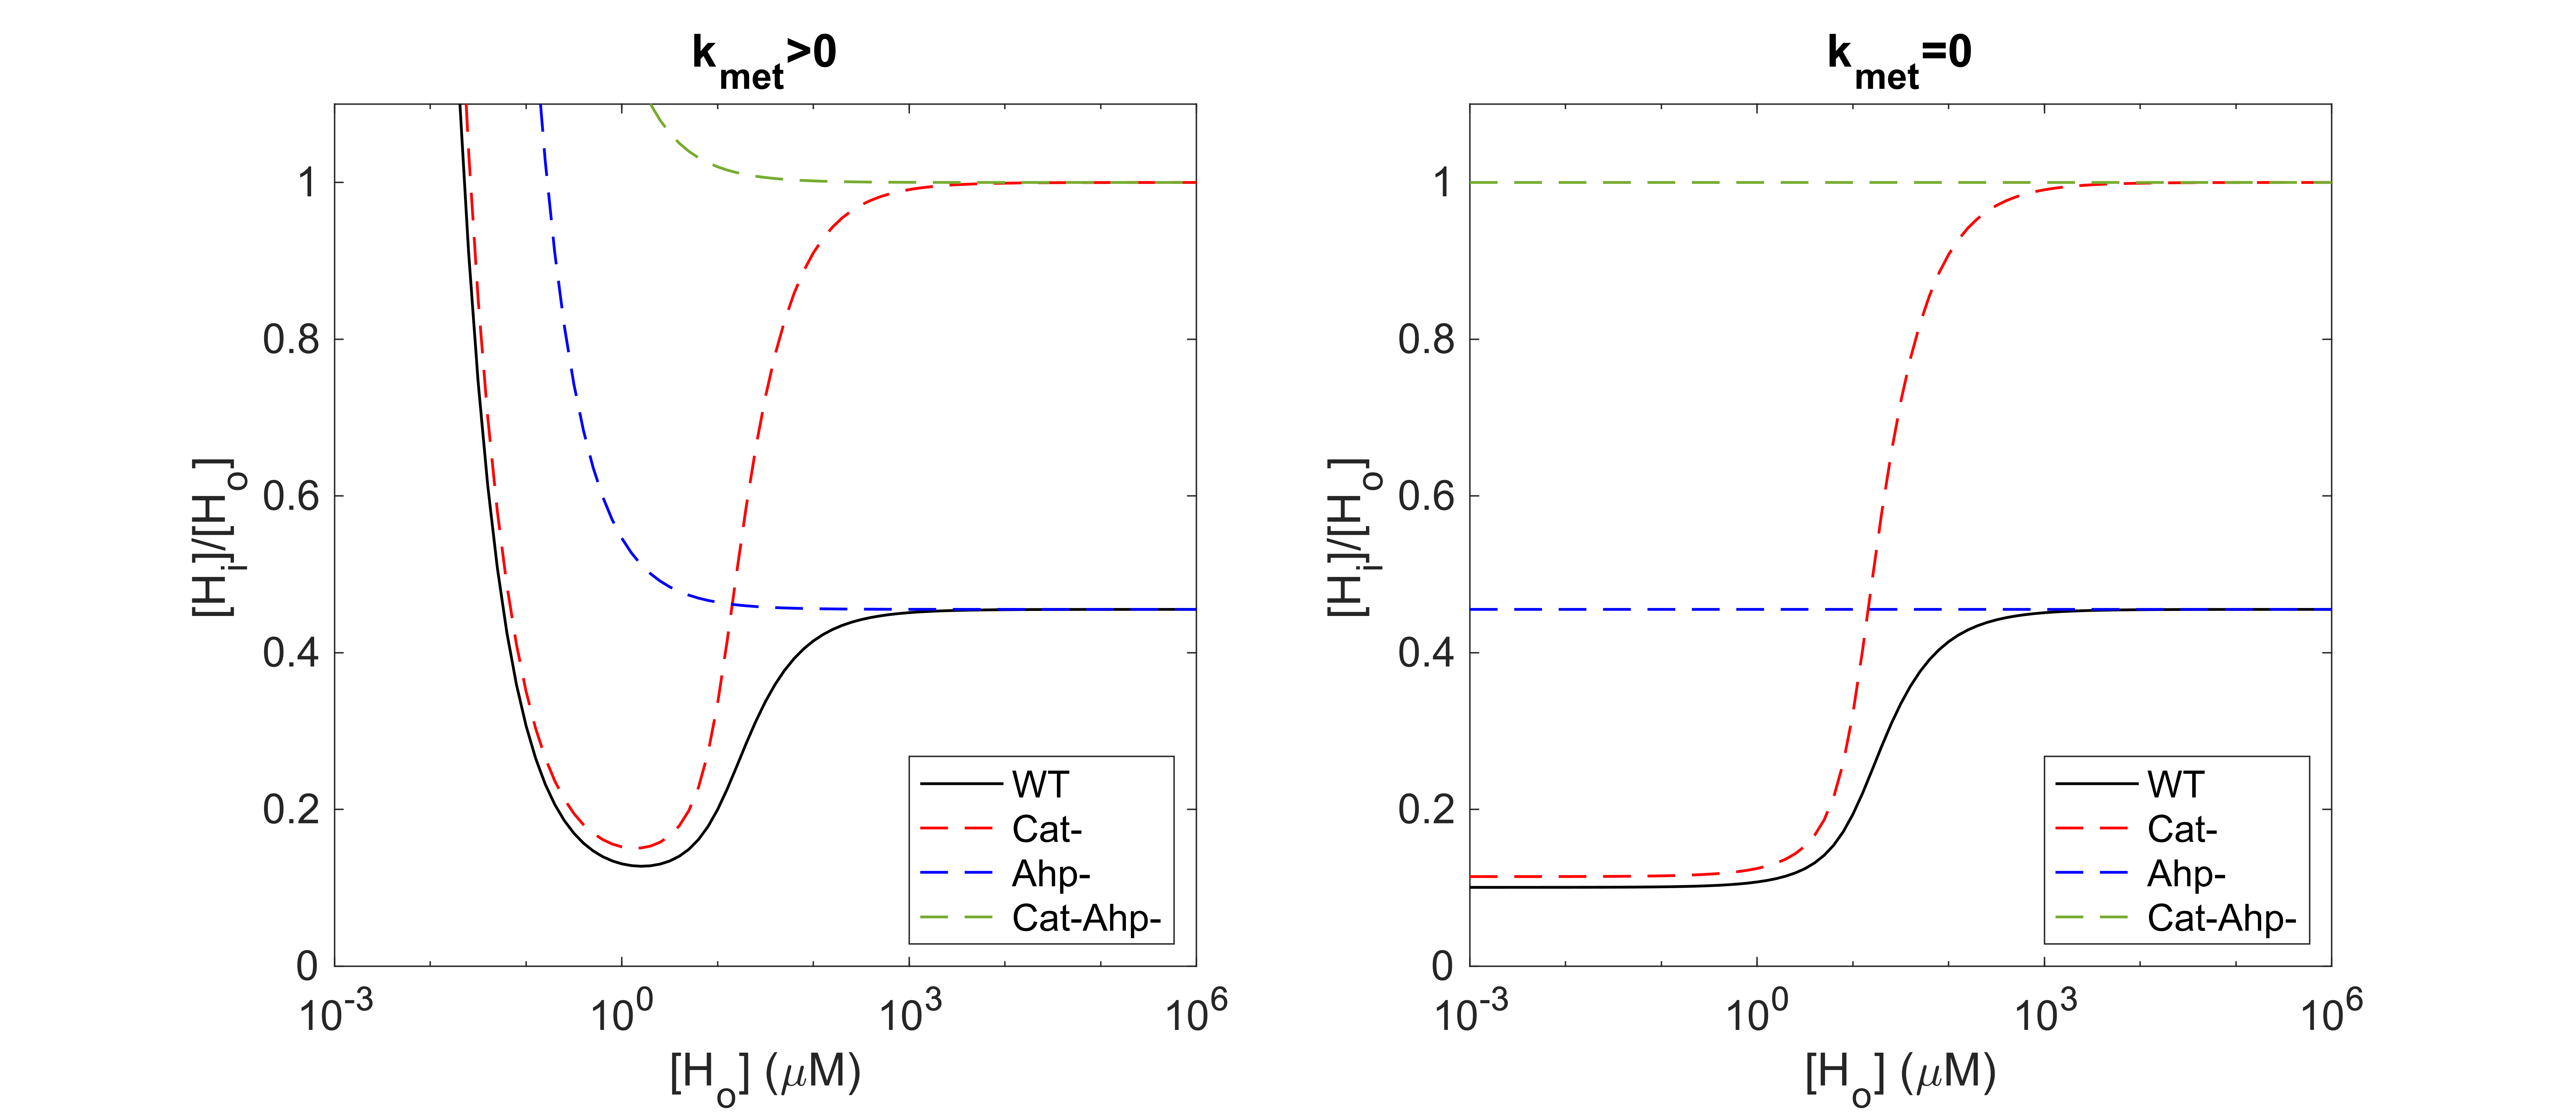
\includegraphics[width=1\linewidth]{HoHi_ratio_mutants.png}
  \caption{Relationship between intracellular and extracellular H2O2 concentrations. (Left panel) H2O2 is produced metabolically. (Right panel) H2O2 is NOT produced metabolically.}
  \label{fig:rHoHi}
\end{figure}

%%%%%%%%%%%%%%%%%%%%
\subsubsection{Response of intracellular H2O2 is biphasic}

When $k_{met}\approx 0$, the $[H_i]/[H_o]$ ratio is bounded between two extremes and increases rapidly when $[H_o]$ passes a certain threshold (Fig.~\ref{fig:rHoHi}, right panel). Interestingly, the lower and upper bound values of the ratio are approximately equal to ratios in Cat- and Ahp- strains, suggesting that the two enzymes play dominant roles in different H2O2 concentration ranges. The lower bound of $[H_i]/[H_o]$ for the wild-type strain can be solved by setting $k_{cat}=0$
\begin{eqnarray}
[H_i] &=& \frac{-\left(K_{m,ahp}-[H_o]+\dfrac{k_{ahp}}{PA}\right)+\sqrt{\left(K_{m,ahp}-[H_o]+\dfrac{k_{ahp}}{PA}\right)^2+4K_{m,ahp}[H_o]}}{2} \\
&=& \frac{K_{m,ahp}}{K_{m,ahp}+\dfrac{k_{ahp}}{PA}}[H_o] + \mathcal{O}([H_o]^2)
\end{eqnarray}
If $[H_o]$ is small, we retain the leading term only, giving
\begin{equation}
\left(\frac{[H_i]}{[H_o]}\right)_{lb} = \dfrac{PA}{PA+\dfrac{k_{ahp}}{K_{m,ahp}}}
\end{equation}
Similarly, the upper bound of the ratio can be derived by setting $k_{ahp}=0$, leading to
\begin{equation}
\left(\frac{[H_i]}{[H_o]}\right)_{ub} = \frac{PA}{PA+k_{cat}}
\end{equation}
\clblue{In sum, the H2O2 concentration gradient across membrane is determined by both cell membrane permeability and specific activity of H2O2-scavenging enzymes. The response of intracellular H2O2 is biphasic, which is originated from the differential H2O2 affinity between catalase and Ahp. This biphasic response has been reported in yeast strain \textit{Saccharomyces pombe}~\cite{tomalin2016increasing}, where H2O2-triggered hyperoxidation of Prx to thioredoxin-resistant, peroxidase-inactive form is a key to direct available thioredoxin to repair damage. In contrast, bacterial 2-Cys Prx, such as the E. coli peroxiredoxin AhpC, are
much less sensitive to hyperoxidation.}

%%%%%%%%%%%%%%%%%%%%%%%%
\subsubsection{Ultrasensitivity of OxyR oxidation to increasing extracellular H2O2 concentration}

OxyR is activated by H2O2 through the oxidation of reactive cysteines. Since OxyR behaves as an autorepressor at the transcriptional level, we assume that the total concentration of OxyR is a constant ($OxyR_t$). The dynamics of interconversion between oxidized ($[OxyR_{ox}]$) and reduced ($[OxyR_{red}]$) forms of OxyR is given by
\begin{equation}
\frac{d[OxyR_{ox}]}{dt} = \frac{k_{oxyr,ox}[OxyR_{red}][H_i]^{n_{oxyr}}}{K_{m,oxyr}^{n_{oxyr}}+[H_i]^{n_{oxyr}}}-k_{oxyr,red}[OxyR_{ox}]
\end{equation}
Using $OxyR_t=[OxyR_{ox}]+[OxyR_{red}]$, the fraction of oxidized form of OxyR can be derived as steady state
\begin{equation}
\frac{[OxyR_{ox}]_{ss}}{OxyR_t} = \frac{[H_i]^{n_{oxyr}}}{[H_i]^{n_{oxyr}}\left(1+\dfrac{k_{oxyr,red}}{k_{oxyr,ox}}\right)+\dfrac{k_{oxyr,red}}{k_{oxyr,ox}}K_{m,oxyr}^{n_{oxyr}}}
\end{equation}
The parameter values can be estimated by fitting experimental data (see Fig.~\ref{fig:fit_oxyr_paras})
\begin{figure}[h!]
\centering
  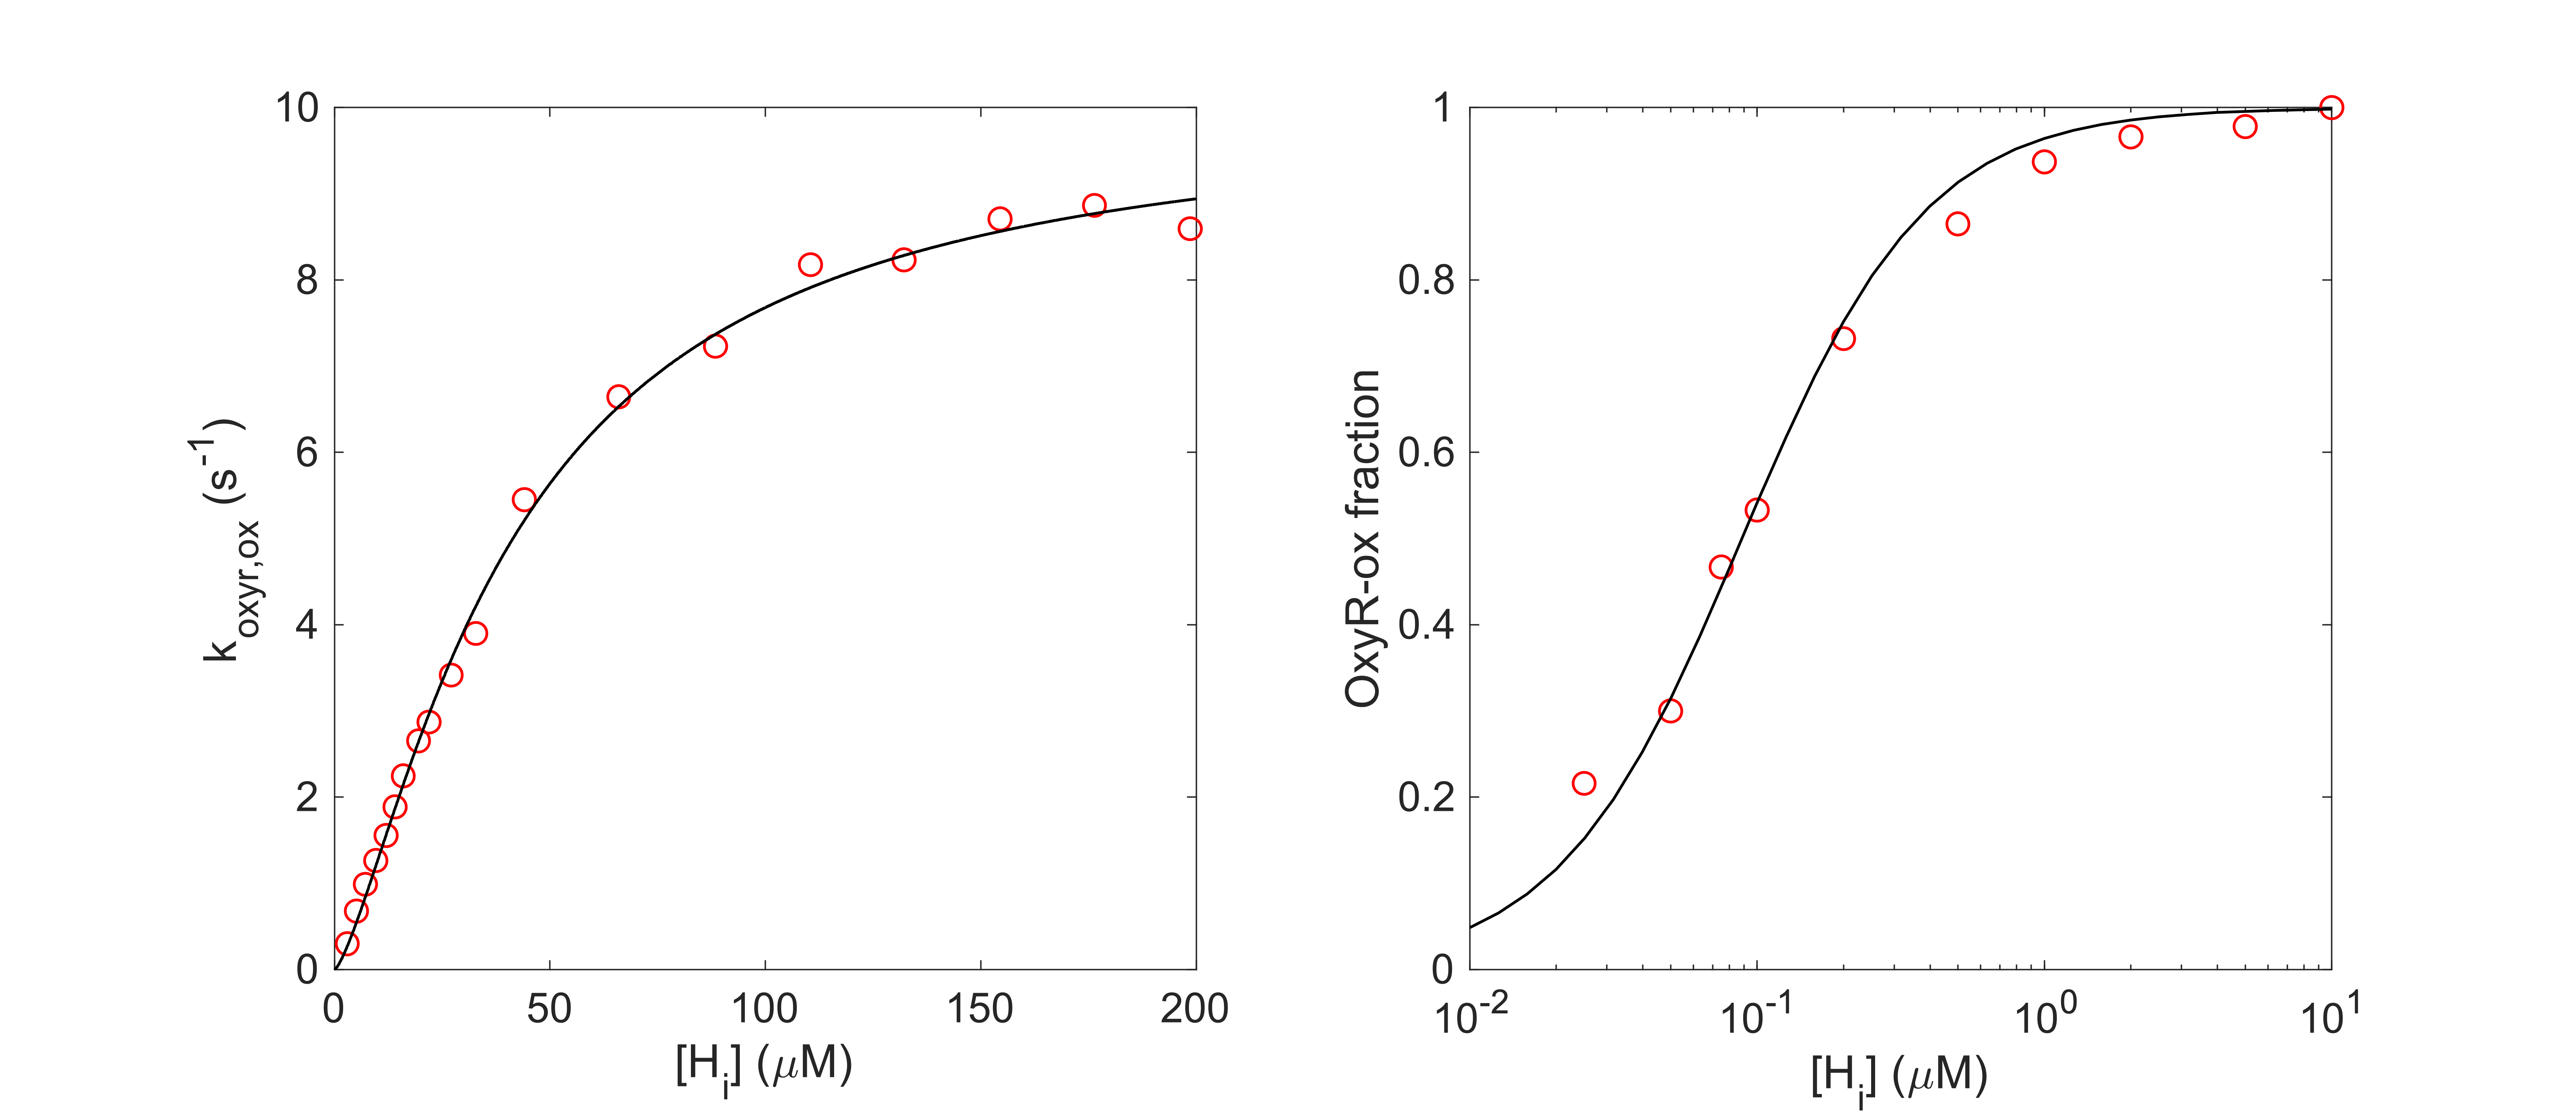
\includegraphics[width=1\linewidth]{fit_oxyR_paras.png}
  \caption{Fitting OxyR-related parameters to experimental data. Data sources: Left panel~\cite{lee2004redox} and right panel~\cite{aaslund1999regulation}. The best-fit parameter values are $n_{oxyr} = 1.36$, $K_{m,oxyr}=41.32~\mu M$, $k_{oxyr,ox}=9.99~s^{-1}$, $k_{oxyr,red}=2.3\times 10^{-3}~s^{-1}$. The value of $k_{oxyr,red}$ corresponds to a half life of 5 min, which is consistent with a previous estimate~\cite{aaslund1999regulation}.}
  \label{fig:fit_oxyr_paras}
\end{figure}

Although the response of OxyR oxidization to increased intracellular H2O2 is Michaelis-Menten-like, its response to extracellular H2O2 is ultrasensitive (Hill coefficient = 10.7)~\cite{pillay2016quantitative}. The fraction of oxidized OxyR increases sharply over a very narrow range of extracellular H2O2 concentration. This switch-like behavior must come from digital-like change of intracellular H2O2 to extracellular H2O2 concentration. We showed below that $K_{m,ahp}$ is a key parameter to generate such discrete state shift. When $K_{m,ahp}$ is a small parameter, we can expand Eq.~\ref{eq:hi_ho} using power series of $K_{m,ahp}$
\begin{equation*}
[H_i] = \begin{cases}
\dfrac{[H_o]PA+k_{met}}{k_{ahp}-[H_o]PA-k_{met}}K_{m,ahp} + \mathcal{O}(K_{m,ahp}^2) & \text{$[H_o]<\dfrac{k_{ahp}-k_{met}}{PA}$}\\
\\
\dfrac{[H_o]PA+k_{met}-k_{ahp}}{PA+k_{cat}} + \dfrac{k_{ahp}}{[H_o]PA+k_{met}-k_{ahp}}K_{m,ahp} + \mathcal{O}(K_{m,ahp}^2) &  \text{$[H_o]\ge\dfrac{k_{ahp}-k_{met}}{PA}$}
\end{cases}
\end{equation*}
The underlying principle is called zero-order ultrasensitivity~\cite{ferrell2014ultrasensitivity}, which occurs under saturation conditions ($K_{m,ahp}\ll[H_i]$). We showed that decreasing $Km_{ahp}$ indeed makes OxyR response more switch-like (Fig.~\ref{fig:fit_oxyRox_parafit}, left panel).

To quantitatively fit the experimental data, we first varied $k_{ahp}$ and $K_{m,ahp}$ at the same time. Although a good fitting can be achieved (Fig.~\ref{fig:fit_oxyRox_parafit}, right panel, dashed line), the best-fit value of $K_{m,ahp}$ is below 1 nM, which is unrealistic. Then we tried fitting $K_{m,ahp}$ alone while fixing $k_{ahp}$ (Fig.~\ref{fig:fit_oxyRox_parafit}, right panel, solid line). The best-fit $K_{m,ahp}$ is 78.66 nM, which is consistent with previous estimation that the intracellular H2O2 concentration is about 50 nM and an intracellular concentration of about 200 nM is sufficient to drive OxyR into the oxidized form~\cite{imlay2013molecular}.

\begin{figure}[h!]
\centering
  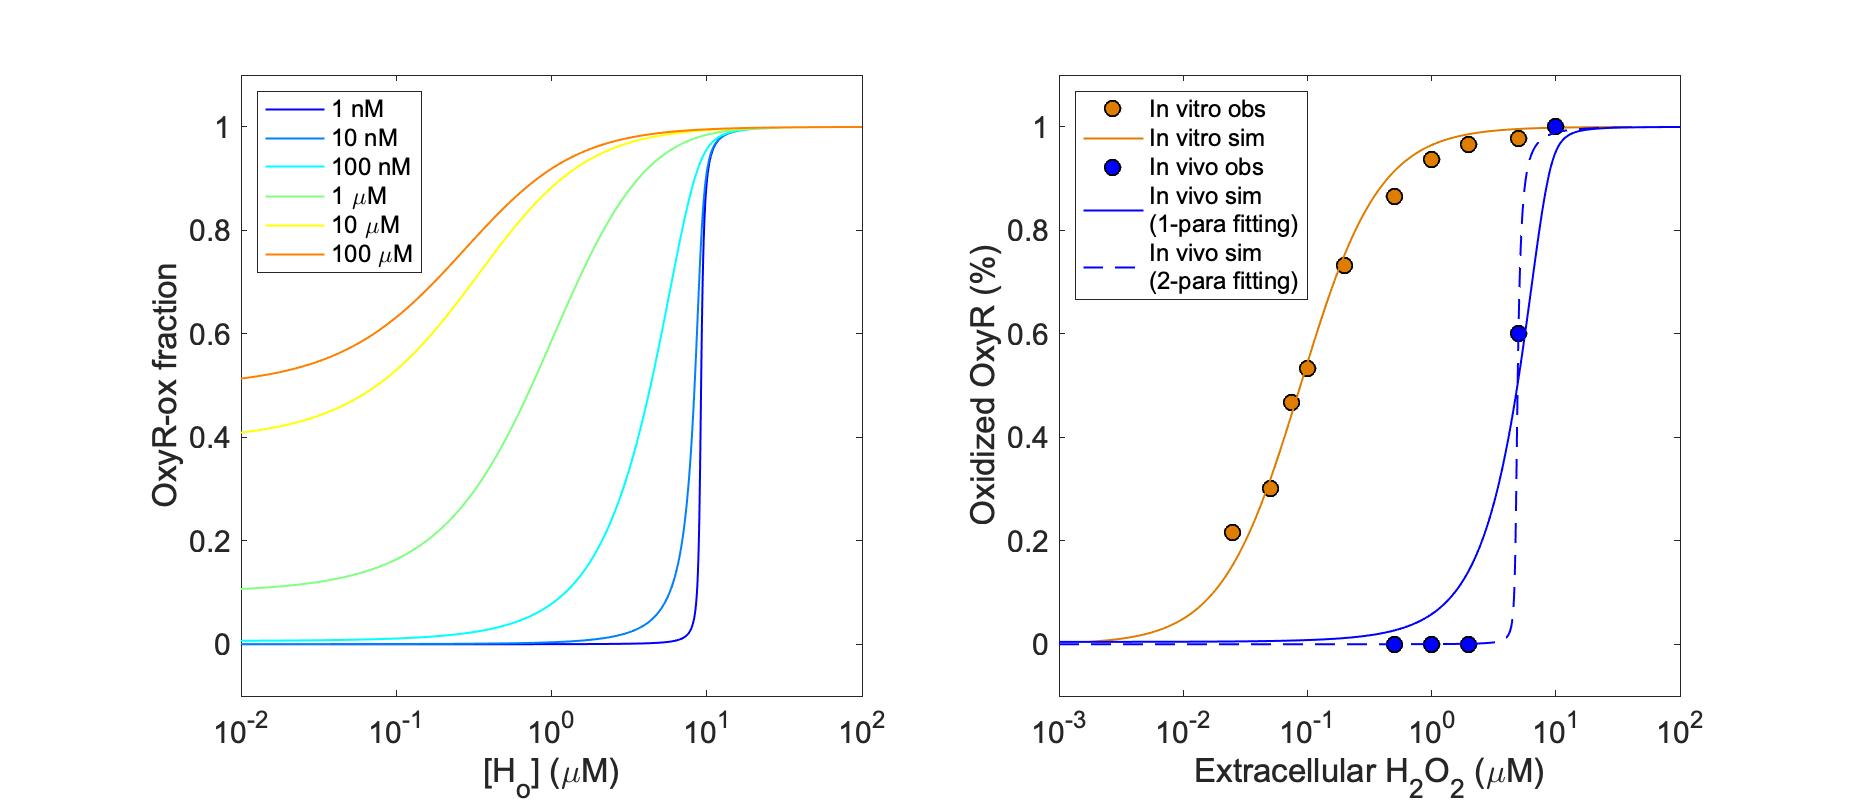
\includegraphics[width=1\linewidth]{fit_oxyRox_1para.png}
  \caption{Single-parameter fitting. (Left panel) OxyR response becomes ultrasensitive with decreased value of $K_{m,ahp}$. (Right panel) Fitting $K_{m,ahp}$ and $k_{ahp}$ to experimental data. For 2-parameter fitting, the best-fit parameter values are $k_{ahp}=1.12\times 10^{-18}~mol/s$ and $K_{m,ahp} = 0.557~nM$. For single-parameter fitting, the best-fit parameter value is $K_{m,ahp} = 78.66~nM$.}
  \label{fig:fit_oxyRox_parafit}
\end{figure}

%%%%%%%%%%%%%%%%%%%%
\subsection{Regulated model (Ahp and KatG expression regulated by OxyR)}
We assume that the synthesis rates of Cat and Ahp are proportional to the fraction of the oxidized OxyR
\begin{eqnarray}
\frac{d[H_i]}{dt} &=& \dfrac{k_{met}+([H_o]-[H_i])PA}{V_c} -k_{0,cat}[Cat][H_i] - \dfrac{k_{0,ahp}[Ahp][H_i]}{K_{m,ahp}+[H_i]}\\
\frac{d[H_o]}{dt} &=& -\frac{([H_o]-[H_i])PA}{V_e} \\
\frac{d[Cat]}{dt} &=& \alpha_{cat}\frac{[H_i]^{n_{oxyr}}}{[H_i]^{n_{oxyr}}\left(1+\dfrac{k_{oxyr,red}}{k_{oxyr,ox}}\right)+\dfrac{k_{oxyr,red}}{k_{oxyr,ox}}K_{m,oxyr}^{n_{oxyr}}}-\lambda[Cat] \\
\frac{d[Ahp]}{dt} &=& \alpha_{ahp}\frac{[H_i]^{n_{oxyr}}}{[H_i]^{n_{oxyr}}\left(1+\dfrac{k_{oxyr,red}}{k_{oxyr,ox}}\right)+\dfrac{k_{oxyr,red}}{k_{oxyr,ox}}K_{m,oxyr}^{n_{oxyr}}}-\lambda[Ahp]
\end{eqnarray}
where $k_{0,cat}$ and $k_{0,ahp}$ are the H2O2 consumption rates per molecule of respective enzymes, $\alpha_{cat}$ and $\alpha_{ahp}$ are the maximum production rates of respective enzymes, and $\lambda$ is the specific growth rate. The following parameter values are used: $k_{0,cat}=4.188\times 10^{6}~(s\cdot M)^{-1}$~\cite{claiborne1979purification}, $k_{0,ahp}=52.4~s^{-1}$~\cite{parsonage2008substrate}, $\alpha_{cat}=3.62\times 10^{-24}~mol/s$~\cite{li2014quantifying}, $\alpha_{ahp}=1.19\times 10^{-22}~mol/s$~\cite{li2014quantifying}, $\lambda=1.93~h^{-1}$~\cite{li2014quantifying} and $V=2~\mu m^3$.

%%%%%%%%%%%%%%%%%
%%%%%%%%%%%%%%%%%
\section{Simple cell growth model}

\subsection{Derivation of a Minimal Cell Growth Model for \textit{E. coli}}

{\color{black}Our kinetic bacterial growth model} defines {\color{black}the interplay between the concentrations of precursor $[P]$, ribosomes $[R]$, the global regulator $[X]$,} and the specific growth rate of the cell $\Lambda$. The dynamics of {\color{black}$[R]$, $[P]$, and $[X]$ are} modeled by {\color{black}considering} the{\color{black}ir} rate{\color{black}s} of production minus the{\color{black}ir} rate{\color{black}s} of consumption and degradation. {\color{black}Namely,}
\begin{eqnarray}
\dfrac{d [P]}{d t} &=&  J_p^{in}-J_p^{out} \label{eq:amino_acid_general_equation}\\
\dfrac{d [R]}{d t} &=&  J_r^{in}-J_r^{out}  \label{eq:ribosome_general_equation} \\
\dfrac{d [X]}{d t} &=&  J_x^{in}-J_x^{out} \label{eq:ppGpp_general_equation}
\end{eqnarray}
{\color{black}where $J_x^{in}$ is the production rate of molecule $x$ and $J_x^{out}$ is its combined consumption and degradation rate.} The specific growth rate is determined {\color{black}with respect to} cell volume $\Omega$, which grows exponentially {\color{black}as}
\begin{equation}\label{eq:growth_rate_general_equation}
\Lambda = \dfrac{1}{\Omega}\dfrac{d \Omega}{d t}
\end{equation}
The mathematical representations of these reaction rates are detailed as follows.

\subsubsection{A coarse-grained model of \textit{E. coli} proteome}

{\color{black}Recent} experimental {\color{black}studies}~\cite{scott2010interdependence,hui2015quantitative} have shown that the proteome of exponentially growing \textit{E. coli} cells can be minimally partitioned into two sectors {\color{black}which each have a distinct role in determining its physiology.} Ribosomal and affiliated proteins {\color{black}belong to the $R$ sector,} catabolic and anabolic enzymes for nutrient uptake and conversion {\color{black}belong to the $E$ sector. Since the \textit{E. coli} mass density is relatively constant in presence of various perturbations~\cite{kubitschek1984independence,basan2015inflating} and the majority of biomass is protein~\cite{bremer2008modulation}, the protein density $[O]$ remains unchanged under different growth conditions. {\color{black}That is,}
\begin{equation}\label{eq:proteome_conservation_REonly}
[O]=m_r[R]+m_e[E] =  \beta
\end{equation}

\subsubsection{The precursor production, consumption and degradation rates}
\label{sect_the_amino_acid_production_consumption_and_degradation_rate}

Under constant or saturating nutrient concentration, the nutrient uptake rate is determined by the availability of metabolic proteins and subject to feedback inhibition by {\color{black}its} end products, {\color{black} precursor. That is, when the metabolic intermediates between nutrient and precursor are ignored,}
\begin{equation}\label{eq:Ja_in_general_equation}
J_p^{in} = f_e([E])\dfrac{[P]}{K_{ip}+[P]}
\end{equation}
where the function $f_e([E])$ {\color{black}relates the influx of precursor to the concentration of coarse-grained metabolic proteins.} For most rate-limiting enzymes that absorb nutrients from environment, the function is linear~\cite{aidelberg2014hierarchy}, {\color{black}so}
\begin{equation}\label{eq:fe_lin}
f_e([E]) = k_e[E]
\end{equation}
where $k_e$ {\color{black}is a linear coefficient that} represents the nutrient quality.

{\color{black}In this framework, }precursors {\color{black}are utilized solely for} protein synthesis {\color{black}and not for} other metabolic reactions. Since each active ribosome is able to initiate translation, the consumption rate of precursor ($J_p^{con}$) in protein synthesis is modelled using a Michaelis-Menten equation
\begin{equation}
J_{con}^p = \frac{k_{r}[R][P]}{K_{mp}+[P]}
\end{equation}

We assume precursors {\color{black}are only diluted via volume expansion,} so
\begin{equation}
J_p^{deg}  = \Lambda[P]
\end{equation}
{\color{black}is the degradation rate.}
The total precursor outflux rate is {\color{black}the} sum of {\color{black}the} reaction rates from both {\color{black}utilization via} protein synthesis and dilution {\color{black}via volume expansion}, that is,
\begin{equation}\label{eq:aminoacid_outflux}
J_p^{out} = J_p^{con} + J_p^{deg} 
\end{equation}

\subsubsection{The ribosome synthesis and degradation rates}

It is generally believed that the synthesis of ribosomal RNAs is the limiting step in ribosome production due to excessive ribosomal proteins than ribosomal RNAs~\cite{gourse1996rrna}. On the other hand, ribosome production is also limited by the synthesis of ribosomal proteins in terms of reaction dynamics because protein synthesis takes much longer time as compared to RNA synthesis. Considering the dynamic nature of our minimal model, we assume the latter, meaning that the ribosome production rate $J_r^{in}$ is determined by the fraction of total translational capacity allocated for producing R sector proteins. {\color{black} Additionally, because ppGpp inhibits transcription initiation of ribosomal proteins both \textit{in vitro} and \textit{in vivo}~\cite{lemke2011direct}, a function $\alpha_r$ that describes the degree of inhibition is included. The ribosome production rate is then}
\begin{equation}\label{eq:ribosome_synthesis_rate}
J_r^{in} = \dfrac{J_p^{con}\alpha_r}{m_r}
\end{equation}
The regulation of ribosome by the global regulatory $X$ is written as a Michaelis-Menten function
\begin{equation}
\alpha_r = \dfrac{K_{ix}}{[X]+K_{ix}}
\end{equation}
where $K_{ix}$ {\color{black}is the regulator concentration at which half of ribosome synthesis is halted.}

Ribosomes are very stable in fast growth {\color{black}but are degraded in starvation, entry into stationary phase, and slow growth}~\cite{piir2011ribosome,deutscher2003degradation}. For simplicity, we assume ribosomes are not degraded but decay due to dilution effect
\begin{equation}\label{eq:ribosome_degradation_rate}
J_r^{out} = \Lambda[R]
\end{equation}

\subsubsection{The synthesis and degradation rates of global regulator}

We assume the synthesis rate of global regulator $X$ is inversely regulated by the precursor concentration
\begin{equation}\label{eq:ppGpp_synthesis_rate}
J_x^{in} = k_x\frac{K_{mp}}{K_{mp}+[P]}
\end{equation}
where $k_x$ {\color{black} is the maximal synthesis rate.}

The turnover rate of global regulator is generally much faster than the decay rate due to dilution. Therefore, we assume first-order active degradation and ignore the dilution effect
\begin{equation} \label{eq:ppGpp_outflux_rate}
J_x^{out} = d_{x}[X]
\end{equation}
where $d_{x}$ is the first order degradation rate constant.

\subsubsection{The specific growth rate}

{\color{black}Using the previous assumption that the intracellular protein density is constant,} the specific growth rate $\Lambda$ {\color{black}is determined by the rate of protein production} 
\begin{equation}\label{eq:relationship_between_lambda_and_Jacon}
\Lambda = \dfrac{1}{\Omega}\dfrac{d \Omega}{d t} = \dfrac{1}{\beta}\left(\dfrac{1}{\Omega}\dfrac{d O}{d t}\right) = \dfrac{J_p^{con}}{\beta}
\end{equation}

\subsubsection{Summary}
\label{sect_summary}

The entire model equations are summarized below

\small
\allowdisplaybreaks[1]
\begin{eqnarray}
 \dfrac{d [(H_2O_2)_{in}]}{d t} &=& \underbrace{k_e[E]}_{\substack{\text{maximum precursor} \\ \text{synthesis rate}}}\underbrace{{\clred{\dfrac{K_{ip}}{K_{ip}+[P]}}}}_{\substack{\text{feedback} \\ \text{inhibition}}}-\underbrace{\dfrac{k_r[R][P]}{K_{mp}+[P]}}_{\substack{\text{precursor}\\ \text{consumption rate}}}-\underbrace{\Lambda[P]}_{\substack{\text{precursor} \\ \text{dilution rate}}} 
\label{eq:metab_prot_conc}
  \end{eqnarray}

\small
\allowdisplaybreaks[1]
\begin{eqnarray}
 \dfrac{d [P]}{d t} &=& \underbrace{k_e[E]}_{\substack{\text{maximum precursor} \\ \text{synthesis rate}}}\underbrace{{\clred{\dfrac{K_{ip}}{K_{ip}+[P]}}}}_{\substack{\text{feedback} \\ \text{inhibition}}}-\underbrace{\dfrac{k_r[R][P]}{K_{mp}+[P]}}_{\substack{\text{precursor}\\ \text{consumption rate}}}-\underbrace{\Lambda[P]}_{\substack{\text{precursor} \\ \text{dilution rate}}} \label{eq:dadt_summary}\\
\dfrac{d [R]}{d t} &=& \underbrace{\frac{k_r[R][P]}{m_r(K_{mp}+[P])}\frac{K_{ix}}{K_{ix}+[X]}}_{\substack{\text{ribosome} \\ \text{synthesis rate}}}-\underbrace{\Lambda[R]}_{\substack{\text{ribosome} \\ \text{dilution rate}}} \label{eq:drdt_summary} \\
  \dfrac{d [X]}{d t} &=& \underbrace{k_x\frac{K_{mp}}{K_{mp}+[P]}}_{\substack{\text{regulator}\\\text{synthesis rate}}}-\underbrace{d_{x}[X]}_{\substack{\text{regulator}\\\text{degradation rate}}} ~\label{eq:dgdt_summary}\\
    \Lambda &=& \underbrace{\dfrac{k_r[R][P]}{\beta(K_{mp}+[P])}}_{\text{specific growth rate}} \label{eq:growth_rate_summary}\\
   ~[E] &=& \underbrace{\dfrac{\beta-m_r[R]}{m_e}}_{\substack{\text{metabolic protein} \\ \text{concentration}}} \label{eq:metab_prot_conc}
  \end{eqnarray}
\subsection{Nondimensionalization}

The following transformations are made:\newline
$p=[P]/\beta$, $r=m_r[R]/\beta$, $x=[X]/\beta$, $\tau=k_r t/m_r$, $\lambda=m_r\Lambda/k_r$, $k_e^\prime=m_rk_e/(k_rm_e)$, $k_x^\prime=(k_xm_r)/(k_r\beta)$, $d_x^\prime = d_xm_r/k_r$, $K_{mp}^\prime = K_{mp}/\beta$, $K_{ix}^\prime = K_{ix}/\beta$, $K_{ip}^{\prime}=K_{ip}/\beta$.

\small
\allowdisplaybreaks[1]
\begin{eqnarray}
\frac{dp}{d\tau} &=& k_e^{\prime}(1-r)\frac{K_{ip}^\prime}{K_{ip}^{\prime}+p}-\lambda(1+p) \label{eq:dpdtau_nd}\\
\frac{dr}{d\tau} &=& \lambda\left(\frac{K_{ix}^{\prime}}{K_{ix}^\prime+x}-r\right) \label{eq:drdtau_nd}\\
\frac{dx}{d\tau} &=& k_x^{\prime}\frac{K_{mp}^{\prime}}{K_{mp}^{\prime}+p}-d_x^{\prime}x \label{eq:dxdtau_nd}\\
\lambda &=& \frac{rp}{K_{mp}^{\prime}+p} \label{eq:lambda_nd}
  \end{eqnarray}

\subsection{Parameters}

\begin{table}[!htbp]
\centering
\small
\setlength\extrarowheight{5pt}
\begin{tabular}{|c|l|c|c|c|c|}
\hline
 \textbf{Symbol} & \textbf{Description} & \textbf{Value}  & \textbf{Unit}  & \textbf{Formula} & \textbf{Source}  \\ \hline
 $m_r$ & \# of precursor in a ribosome & $11738$ & & $7336\times1.6$ & \cite{klumpp2013molecular} \\ \hline
 $m_e$ & \# of precursor in a metabolic protein & $325$ &   & & \cite{maitra2015bacterial} \\ \hline
 $k_r$ & maximum rate of peptide elongation & $7.56\times 10^4$ & \unitfrac{1}{hr} & $\unitfrac[21]{1}{s} \times \unitfrac[3600]{s}{hr}$ & \cite{marr1991growth} \\ \hline
 $k_x$ & maximum rate of ppGpp synthesis &  $3.6\times 10^{3}$ & \unitfrac{1}{hr} & $\unitfrac[1]{1}{s} \times \unitfrac[3600]{s}{hr}$   & \cite{marr1991growth} \\ \hline
 $d_x$ &  first-order rate constant of ppGpp degradation & $1.26\times 10^{2}$ & \unitfrac{1}{hr} & $\unitfrac[0.035]{1}{s} \times \unitfrac[3600]{s}{hr}$ & \cite{marr1991growth} \\ \hline
 $K_{mp}$ & dissociation constant for amino acid & $2.00\times 10^{1}$ & $\mu M$ & & \cite{marr1991growth} \\ \hline
 $K_{ix}$ & dissociation constant for ppGpp & $6.00\times10^{1}$ & $\mu M$ & & \\ \hline
 $\beta$ & total peptide concentration & $3.00\times 10^6$ & $\mu M$ & & \cite{marr1991growth} \\ \hline
 $K_{ip}$ & precursor feedback inhibition constant & $1.00\times 10^{4}$ & $\mu M$ & & \\ \hline
\end{tabular}
\caption{Model parameters used in the model.}
\label{tab:parameters}
\end{table}
\normalsize

\subsection{Steady state solution}

Let $p \ll K_{ip}^\prime$ so that $K_{ip}^{\prime}/(K_{ip}^{\prime}+p) \approx 1$. Combining Eq.~\ref{eq:dpdtau_nd} and Eq.~\ref{eq:lambda_nd} gives
\begin{equation}
\lambda = \frac{k_e^{\prime}}{1+p+k_e^{\prime}\dfrac{K_{mp}^{\prime}+p}{p}}
\end{equation}
Similarly, combining Eq.~\ref{eq:drdtau_nd} and Eq.~\ref{eq:dxdtau_nd} gives
\begin{equation}
\lambda = \frac{K_{ix}^{\prime}p}{K_{ix}^{\prime}(K_{mp}^{\prime}+p)+\dfrac{k_x^{\prime}K_{mp}^{\prime}}{d_x^{\prime}}}
\end{equation}
Combining the two equations above gives $p^2+p-\frac{k_e^{\prime}k_x^{\prime}K_{mp}^{\prime}}{K_{ix}^{\prime}d_x^{\prime}}=0$, whose solution is given by
\begin{equation}
p=\frac{-1+\sqrt{1+\dfrac{4k_e^{\prime}k_x^{\prime}K_{mp}^{\prime}}{K_{ix}^{\prime}d_x^{\prime}}}}{2}
\end{equation}
Accordingly, the growth rate $\lambda$ is rewritten as
\begin{equation}
\lambda = \frac{k_e^{\prime}}{k_e^{\prime}+\dfrac{1}{2}\left(1+\sqrt{1+\dfrac{4k_e^{\prime}k_x^{\prime}K_{mp}^\prime}{K_{ix}^{\prime}d_x^{\prime}}}\right)\left(1+\dfrac{K_{ix}^{\prime}d_x^{\prime}}{k_x^{\prime}}\right)}
\end{equation}

\section{Cell growth model with fermentation and ATP limitation}

\subsection{Derivation of a cell growth model for \textit{E.coli} with fermentation and ATP limitation}
Two more variables are introduced to account for the fermentation and overflow. $[A_{ex}]$ represents the fermentation product inside the cell. We also assumes that the growth rate can be carbon limited/precursor limited or ATP limited. So the growth rate is the minimum of carbon limited growth rate and ATP limited growth rate. Further, the precursor consumption rate is also assumed to be dependent on the ATP flux. The model equations with fermentation and ATP limitation are as follows:
\footnotesize
\allowdisplaybreaks[1]
\begin{eqnarray*}
%\underbrace{k_e[E]}_{\substack{\text{maximum precursor} \\ \text{synthesis rate}}}
% 	\dfrac{d [P]}{d t} &=& \underbrace{k_e[E]}_{\substack{\text{maximum precursor} \\ \text{synthesis rate}}}\underbrace{{\clred{\dfrac{K_{ip}}{K_{ip}+[P]}}}}_{\substack{\text{feedback} \\ \text{inhibition}}}-\underbrace{\dfrac{k_r[R][P]}{K_{mp}+[P]}}_{\substack{\text{precursor}\\ \text{consumption rate}}}  -\underbrace{\Lambda[P]}_{\substack{\text{precursor} \\ \text{dilution rate}}} \nonumber \\
% &-&\underbrace{\dfrac{v_a[P](1-\dfrac{1}{K_{ca}}\dfrac{[A_{ex}]}{[P]})}{K_{ma}+[P](1+k_{ra}\dfrac{1}{K_{ca}}\dfrac{[A_{ex}]}{[P]})}}_{\substack{\text{reversible fermentation rate} \\ \text{with thermodynamic constrait}}}+\underbrace{\dfrac{k_u[E][A_{ex}]}{K_{mu}+[A_{ex}]}}_{\substack{\text{fermentation product} \\ \text{uptake rate}}} \label{eq:dadt_summary1}\\
  	\dfrac{d [P]}{d t} &=& \underbrace{\frac{k_e[E][S_{ex}]}{K_{ms}+[S_{ex}]}}_{\substack{\text{maximum precursor} \\ \text{synthesis rate}}}\underbrace{{\clred{\dfrac{K_{ip}}{K_{ip}+[P]}}}}_{\substack{\text{feedback} \\ \text{inhibition}}}-\underbrace{\beta \Lambda}_{\substack{\text{precursor}\\ \text{consumption rate}}}  -\underbrace{\Lambda[P]}_{\substack{\text{precursor} \\ \text{dilution rate}}} -\underbrace{\dfrac{v_a[P]\left(1-\dfrac{1}{K_{ca}}\dfrac{[A_{ex}]}{[P]}\right)}{K_{ma}+[P]\left(1+k_{ra}\dfrac{1}{K_{ca}}\dfrac{[A_{ex}]}{[P]}\right)}}_{\substack{\text{reversible fermentation rate} \\ \text{with thermodynamic constrait}}}+\underbrace{\dfrac{k_u[E][A_{ex}]}{K_{mu}+[A_{ex}]}}_{\substack{\text{fermentation product} \\ \text{uptake rate}}}-\underbrace{\dfrac{k_o[E][P]}{K_{mo}+[P]}}_{\substack{\text{rate of} \\ \text{TCA cycle}}} \label{eq:dadt_summary1}\\
	\dfrac{d [R]}{d t} &=& \underbrace{\frac{\beta \Lambda}{m_r}\frac{K_{ix}}{K_{ix}+[X]}}_{\substack{\text{ribosome} \\ \text{synthesis rate}}}-\underbrace{\Lambda[R]}_{\substack{\text{ribosome} \\ \text{dilution rate}}} \label{eq:drdt_summary1} \\
	\dfrac{d [X]}{d t} &=& \underbrace{k_x\frac{K_{mp}}{K_{mp}+[P]}}_{\substack{\text{regulator}\\\text{synthesis rate}}}-\underbrace{d_{x}[X]}_{\substack{\text{regulator}\\
 \text{degradation rate}}} ~\label{eq:dgdt_summary1}\\
%	\dfrac{d [A_{ex}]}{d t} &=& \underbrace{\dfrac{v_a[P](1-\dfrac{1}{K_{ca}}\dfrac{[A_{ex}]}{[P]})}{K_{ma}+[P](1+k_{ra}\dfrac{1}{K_{ca}}\dfrac{[A_{ex}]}{[P]})}}_{\substack{\text{reversible fermentation rate} \\ \text{with thermodynamic constrait}}}-\underbrace{\dfrac{k_u[E][A_{ex}]}{K_{mu}+[A_{ex}]}}_{\substack{\text{fermentation product} \\ \text{uptake rate}}} -\underbrace{\Lambda [A_{ex}]}_{\substack{\text{fermentation product} \\ \text{dilution rate}}} \\
	\Lambda_{b} &=& \underbrace{\dfrac{k_r[R][P]}{\beta(K_{mp}+[P])}}_{\substack{\text{carbon limited growth rate}}} \label{eq:growth_rate_summary1}\\
	\Lambda_{e} &=& \underbrace{\sigma \left(n_p\frac{k_e[E][S_{ex}]}{K_{ms}+[S_{ex}]}\dfrac{K_{ip}}{K_{ip}+[P]}+n_a\left(\dfrac{v_a[P]\left(1-\dfrac{1}{K_{ca}}\dfrac{[A_{ex}]}{[P]}\right)}{K_{ma}+[P]\left(1+k_{ra}\dfrac{1}{K_{ca}}\dfrac{[A_{ex}]}{[P]}\right)}-\dfrac{k_u[E][A_{ex}]}{K_{mu}+[A_{ex}]}\right)+n_o\dfrac{k_o[E][P]}{K_{mo}+[P]}\right)}_{\substack{\text{ATP limited growth rate}}} \label{eq:growth_rate_summary11}\\
%	\Lambda &=& min\{\underbrace{\dfrac{k_r[R][P]}{\beta(K_{mp}+[P])}}_{\substack{\text{carbon limited} \\ \text{growth rate}}} \label{eq:growth_rate1_summary},\underbrace{n_pk_e[E]\dfrac{K_{ip}}{K_{ip}+[P]}+n_a\dfrac{v_a[P](1-\dfrac{1}{K_{ca}}\dfrac{A_{ex}}{P})}{K_{mp}+[P](1+k_{ra}\dfrac{1}{K_{ca}}\dfrac{A_{ex}}{P})}}_{\substack{\text{ATP limited} \\ \text{growth rate}}} \label{eq:growth_rate1_summary}\}\\
	\Lambda &=& \min\{\Lambda_{b}, \Lambda_{e}\} \\ 
   ~[E] &=& \underbrace{\dfrac{\beta-m_r[R]}{m_e}}_{\substack{\text{metabolic protein} \\ \text{concentration}}} \label{eq:metab_prot_conc1}
  \end{eqnarray*}
  
\subsection{Nondimensionalization}
The transformations are as follows:
$p=[P]/\beta$, $r=m_r[R]/\beta$, $x=[X]/\beta$, $\tau=k_r t/m_r$, $\lambda=m_r\Lambda/k_r$, $k_e^\prime=m_rk_e/(k_rm_e)$, $k_x^\prime=(k_xm_r)/(k_r\beta)$, $d_x^\prime = d_xm_r/k_r$, $K_{mp}^\prime = K_{mp}/\beta$, $K_{ix}^\prime = K_{ix}/\beta$, $K_{ip}^{\prime}=K_{ip}/\beta$, $v_a^\prime=m_rv_a/(k_r\beta)$, $K_{ma}^\prime=K_{ma}/\beta$,  $k_{u}^{\prime}=m_rk_u/(k_rm_e)$, $K_{mu}^{\prime}=K_{mu}/\beta$, $n_p^\prime=\sigma  \beta n_p$, $n_a^\prime=\sigma  \beta n_a$.

\small
\allowdisplaybreaks[1]
\begin{eqnarray}
%\frac{dp}{d\tau} &=& k_e^{\prime}(1-r)\frac{K_{ip}^\prime}{K_{ip}^{\prime}+p}-\lambda_b-\lambda p-\frac{v_a^{\prime}p\left(1-\dfrac{1}{K_{ca}}\dfrac{A_{ex}}{p}\right)}{K_{ma}^{\prime}+p\left(1+\dfrac{k_{ra}}{K_{ca}}\dfrac{A_{ex}}{p}\right)} +\frac{k_u^{\prime}(1-r) A_{ex}}{K_{mu}^{\prime}+A_{ex}} \label{eq1:dpdtau_nd1}\\
\frac{dp}{d\tau} &=& k_e^{\prime}(1-r)\frac{K_{ip}^\prime}{K_{ip}^{\prime}+p}-\lambda-\lambda p-\frac{v_a^{\prime}p\left(1-\dfrac{1}{K_{ca}}\dfrac{A_{ex}}{p}\right)}{K_{ma}^{\prime}+p\left(1+\dfrac{k_{ra}}{K_{ca}}\dfrac{A_{ex}}{p}\right)} +\frac{k_u^{\prime}(1-r) A_{ex}}{K_{mu}^{\prime}+A_{ex}} \label{eq1:dpdtau_nd1}\\
\frac{dr}{d\tau} &=& \lambda\frac{K_{ix}^{\prime}}{K_{ix}^\prime+x}-\lambda r \label{eq:drdtau_nd1}\\
\frac{dx}{d\tau} &=& k_x^{\prime}\frac{K_{mp}^{\prime}}{K_{mp}^{\prime}+p}-d_x^{\prime}x \label{eq:dxdtau_nd1}\\
\frac{dA_{ex}}{d\tau} &=& \frac{v_a^{\prime}p\left(1-\dfrac{1}{K_{ca}}\dfrac{A_{ex}}{p}\right)}{K_{ma}^{\prime}+p\left(1+\dfrac{k_{ra}}{K_{ca}}\dfrac{A_{ex}}{p}\right)} -\frac{k_u^{\prime}(1-r) A_{ex}}{K_{mu}^{\prime}+A_{ex}}-\lambda A_{ex}\\
\lambda_b &=& \frac{rp}{K_{mp}^\prime+p} \\
\lambda_e &=& n_p^{\prime}k_e^{\prime}(1-r)\frac{K_{ip}^\prime}{K_{ip}^{\prime}+p} +n_a^{\prime} \frac{v_a^{\prime}p\left(1-\dfrac{1}{K_{ca}}\dfrac{A_{ex}}{p}\right)}{K_{ma}^{\prime}+p\left(1+\dfrac{k_{ra}}{K_{ca}}\dfrac{A_{ex}}{p}\right)}\\
\lambda &=& \min\{\lambda_b, \lambda_e\}
  \end{eqnarray}
  
  \subsection{Parameters}
  \begin{table}[!htbp]
\centering
\tiny
\setlength\extrarowheight{5pt}
\begin{tabular}{|c|l|c|c|l|}
\hline
 \textbf{Symbol} & \textbf{Description} & \textbf{Value}  & \textbf{Unit}  & \textbf{Source}  \\ \hline
 $k_e$ & maximum rate of glucose uptake      & $8.67\times 10^3$   &  $h^{-1}$  & estimated from Enjalbert \textit{et al.}, 2017\\ \hline
 $K_{ms}$ & Michaelis constant for glucose uptake & $6.67$ & $\mu M$ & Jahan \textit{et al.}, 2016\\ \hline
 $m_r$ & \# of aa. (precursor) in a ribosome   & $11738~(7336\times1.6)$ & & Bremer and Dennis, 2008  \\ \hline
 $m_e$ & \# of aa. (precursor) in a metabolic protein & $325$           & & Maitra \textit{et al.}, 2015 \\ \hline
 $k_r$ & maximum rate of peptide elongation & $7.56\times 10^4$   & $h^{-1}$ & Marr, 1991 \\ \hline
 $k_x$ & maximum rate of ppGpp (regulator) synthesis   &  $3.6\times 10^{3}$  & $h^{-1}$  & Marr, 1991 \\ \hline
 $d_x$ &  first-order rate constant of ppGpp (regulator) degradation & $1.26\times 10^{2}$ & $h^{-1}$ & Marr, 1991 \\ \hline
 $K_{mp}$ & dissociation constant for aa. (precursor) & $2.00\times 10^{1}$ & $\mu M$ & Marr, 1991 \\ \hline
 $K_{ix}$ & dissociation constant for ppGpp (regulator) & $6.00\times10^{1}$ & $\mu M$ & assumed \\ \hline
 $\beta$ & total aa. (precursor) concentration & $3.00\times 10^6$ & $\mu M$ & Marr, 1991 \\ \hline
 $K_{ip}$ & aa. (precursor) feedback inhibition constant & $1.00\times 10^{4}$ & $\mu M$ & assumed\\ \hline
 $v_a$ & maximum rate of acetate (fermentation product) production & $1.62\times 10^{8}$ & $\mu M/h$&  Jahan \textit{et al.}, 2016\\ \hline
 $K_{ma}$ & Michaelis constant for acetate (fermentation product) production& $1.60\times 10^{2}$ & $\mu M$ & Jahan \textit{et al.}, 2016\\ \hline
  $K_{ca}$ & equilibrium constant & $4.88\times 10^1$ &  & estimated from Enjalbert \textit{et al.}, 2017 \\ \hline
 $k_{ra}$ & ratio between maximal forward and reverse rate & $1.00$ & $\mu M$ & assumed \\ \hline
 $k_u$ & maximum rate of acetate (fermentation production) reuptake & $9.80\times 10^3$ &  $h^{-1}$ & estimated from Enjalbert \textit{et al.}, 2017 \\ \hline
 $K_{mu}$ & Michaelis constant for acetate (fermentation product) reuptake & $1.67\times 10^{1}$ & $\mu M$ & Jahan \textit{et al.}, 2016\\ \hline
 $P\mathord{:}O$ & ATP produced per NADH or FADH\textsubscript{2} & $2.02$  & & estimated from Enjalbert \textit{et al.}, 2017 \\ \hline
 $n_p$ & ATP yield of glycolysis & $10.08$ & & $2+4(P\mathord{:}O$)  \\ \hline
 $n_a$ & ATP yield of fermentation & $1$ & & $1+0(P\mathord{:}O$)\\ \hline
 $n_r$ & ATP yield of TCA & $9.08$ & & $1+4(P\mathord{:}O)$ \\ \hline
 $\sigma$  & growth rate per ATP production flux & $8.87\times 10^{-9}$ & $\mu M^{-1}$ & Jahan \textit{et al.}, 2016 \\ \hline
\end{tabular}
\caption{Model parameters used in the model.}
\label{tab:parameters}
\end{table}
\normalsize
  
  
  
\section{Cell growth model with fermentation and overflow}

\subsection{Derivation of a cell growth model for \textit{E.coli} with fermentation and overflow}
Two more variables are introduced to account for the fermentation and overflow. $[A_{ex}]$ represents the fermentation product inside the cell. $[A_{ex}]$ is the same fermentaion production outside the cell. The $N$ represents the cell number. 
The model equations with fermentation and overflow are as follows:
\small
\allowdisplaybreaks[1]
\begin{eqnarray}
%\underbrace{k_e[E]}_{\substack{\text{maximum precursor} \\ \text{synthesis rate}}}
 	\dfrac{d N}{d t} &=& \underbrace{\Lambda N}_{\text{growth rate}} - \underbrace{\delta N}_{\text{dilution rate}} \\
  	\dfrac{d [P]}{d t} &=& \underbrace{k_e[E]}_{\substack{\text{maximum precursor} \\ \text{synthesis rate}}}\underbrace{{\clred{\dfrac{K_{ip}}{K_{ip}+[P]}}}}_{\substack{\text{feedback} \\ \text{inhibition}}}-\underbrace{\beta \Lambda}_{\substack{\text{precursor}\\ \text{consumption rate}}}  -\underbrace{\Lambda[P]}_{\substack{\text{precursor} \\ \text{dilution rate}}} \nonumber \\
 &-&\underbrace{\dfrac{v_a[P](1-\dfrac{1}{K_{ca}}\dfrac{[A_{in}]}{[P]})}{K_{mp}+[P](1+k_{ra}\dfrac{1}{K_{ca}}\dfrac{[A_{in}]}{[P]})}}_{\substack{\text{reversible fermentation rate} \\ \text{with thermodynamic constrait}}}+\underbrace{\dfrac{k_u[E][A_{in}]}{K_{mu}+[A_{in}]}}_{\substack{\text{fermentation product} \\ \text{uptake rate}}} \label{eq:dadt_summary2}\\
	\dfrac{d [R]}{d t} &=& \underbrace{\frac{\beta \Lambda}{m_r}\frac{K_{ix}}{K_{ix}+[X]}}_{\substack{\text{ribosome} \\ \text{synthesis rate}}}-\underbrace{\Lambda[R]}_{\substack{\text{ribosome} \\ \text{dilution rate}}} \label{eq:drdt_summary2} \\
	\dfrac{d [X]}{d t} &=& \underbrace{k_x\frac{K_{mp}}{K_{mp}+[P]}}_{\substack{\text{regulator}\\\text{synthesis rate}}}-\underbrace{d_{x}[X]}_{\substack{\text{regulator}\\
 \text{degradation rate}}} ~\label{eq:dgdt_summary2}\\
	\dfrac{d [A_{in}]}{d t} &=& \underbrace{\dfrac{v_a[P](1-\dfrac{1}{K_{ca}}\dfrac{[A_{in}]}{[P]})}{K_{mp}+[P](1+k_{ra}\dfrac{1}{K_{ca}}\dfrac{[A_{in}]}{[P]})}}_{\substack{\text{reversible fermentation rate} \\ \text{with thermodynamic constrait}}}-\underbrace{\dfrac{k_u[E][A_{in}]}{K_{mu}+[A_{in}]}}_{\substack{\text{fermentation product} \\ \text{uptake rate}}}+ \underbrace{D([A_{ex}]-[A_{in}])}_{\substack{\text{diffusion of} \\ \text{fermentation product}}} - \underbrace{\Lambda [A_{in}]}_{\text{dilution rate}}\\
	\dfrac{d [A_{ex}]}{d t} &=& \underbrace{-D([A_{ex}]-[A_{in}])(\frac{V_cN}{V_m})}_{\substack{\text{diffusion of} \\ \text{fermentation product}}} - \underbrace{\delta [A_{ex}]}_{\substack{\text{dilution of extracellular} \\ \text{fermentation product}}}\\
	\Lambda_{b} &=& \underbrace{\dfrac{k_r[R][P]}{\beta(K_{mp}+[P])}}_{\substack{\text{carbon limited} \\ \text{growth rate}}} \label{eq:growth_rate_summary2}\\
	\Lambda_{e} &=& \underbrace{n_pk_e[E]\dfrac{K_{ip}}{K_{ip}+[P]}+n_a\dfrac{v_a[P](1-\dfrac{1}{K_{ca}}\dfrac{[A_{ex}]}{[P]})}{K_{mp}+[P](1+k_{ra}\dfrac{1}{K_{ca}}\dfrac{[A_{ex}]}{[P]})}}_{\substack{\text{ATP limited} \\ \text{growth rate}}} \label{eq:growth_rate_summary22}\\
%	\Lambda &=& min\{\underbrace{\dfrac{k_r[R][P]}{\beta(K_{mp}+[P])}}_{\substack{\text{carbon limited} \\ \text{growth rate}}} \label{eq:growth_rate1_summary},\underbrace{n_pk_e[E]\dfrac{K_{ip}}{K_{ip}+[P]}+n_a\dfrac{v_a[P](1-\dfrac{1}{K_{ca}}\dfrac{A_{ex}}{P})}{K_{mp}+[P](1+k_{ra}\dfrac{1}{K_{ca}}\dfrac{A_{ex}}{P})}}_{\substack{\text{ATP limited} \\ \text{growth rate}}} \label{eq:growth_rate1_summary}\}\\
	\Lambda &=& min\{\Lambda_{b}, \Lambda_{e}\} \\ 
   ~[E] &=& \underbrace{\dfrac{\beta-m_r[R]}{m_e}}_{\substack{\text{metabolic protein} \\ \text{concentration}}} \label{eq:metab_prot_conc2}
  \end{eqnarray}
  
  \subsection{Nondimensionlization}
  The transformations are as follows:
$p=[P]/\beta$, $r=m_r[R]/\beta$, $x=[X]/\beta$, $a_{in}=A_{in}/\beta$, $a_{ex}=A_{ex}/\beta$, $\tau=k_r t/m_r$, $\lambda=m_r\Lambda/k_r$, $k_e^\prime=m_rk_e/(k_rm_e)$, $k_x^\prime=(k_xm_r)/(k_r\beta)$, $d_x^\prime = d_xm_r/k_r$, $K_{mp}^\prime = K_{mp}/\beta$, $K_{ix}^\prime = K_{ix}/\beta$, $K_{ip}^{\prime}=K_{ip}/\beta$, $v_a^\prime=m_rv_a/(k_r\beta)$, $K_{ma}^\prime=K_{ma}/\beta$,  $k_{u}^{\prime}=m_rk_u/(k_rm_e)$, $K_{mu}^{\prime}=K_{mu}/\beta$, $n_p^\prime=\sigma  \beta n_p$, $n_a^\prime=\sigma  \beta n_a$, $ \delta^\prime= m_r \delta/k_r$, $ D^\prime= m_r D/k_r$.

\small
\allowdisplaybreaks[1]
\begin{eqnarray}
%\frac{dp}{d\tau} &=& k_e^{\prime}(1-r)\frac{K_{ip}^\prime}{K_{ip}^{\prime}+p}-\lambda_b-\lambda p-\frac{v_a^{\prime}p\left(1-\dfrac{1}{K_{ca}}\dfrac{A_{ex}}{p}\right)}{K_{ma}^{\prime}+p\left(1+\dfrac{k_{ra}}{K_{ca}}\dfrac{A_{ex}}{p}\right)} +\frac{k_u^{\prime}(1-r) A_{ex}}{K_{mu}^{\prime}+A_{ex}} \label{eq1:dpdtau_nd1}\\
\frac{dN}{d\tau} &=& \lambda N - \delta^\prime N \label{eq1:dndtau_nd2}\\
\frac{dp}{d\tau} &=& k_e^{\prime}(1-r)\frac{K_{ip}^\prime}{K_{ip}^{\prime}+p}-\lambda-\lambda p-\frac{v_a^{\prime}p\left(1-\dfrac{1}{K_{ca}}\dfrac{a_{in}}{p}\right)}{K_{ma}^{\prime}+p\left(1+\dfrac{k_{ra}}{K_{ca}}\dfrac{a_{in}}{p}\right)} +\frac{k_u^{\prime}(1-r) A_{ex}}{K_{mu}^{\prime}+a_{in}} \label{eq1:dpdtau_nd2}\\
\frac{dr}{d\tau} &=& \lambda\frac{K_{ix}^{\prime}}{K_{ix}^\prime+x}-\lambda r \label{eq:drdtau_nd2}\\
\frac{dx}{d\tau} &=& k_x^{\prime}\frac{K_{mp}^{\prime}}{K_{mp}^{\prime}+p}-d_x^{\prime}x \label{eq:dxdtau_nd2}\\
\frac{da_{in}}{d\tau} &=& \frac{v_a^{\prime}p\left(1-\dfrac{1}{K_{ca}}\dfrac{a_{in}}{p}\right)}{K_{ma}^{\prime}+p\left(1+\dfrac{k_{ra}}{K_{ca}}\dfrac{a_{in}}{p}\right)} -\frac{k_u^{\prime}(1-r) a_{in}}{K_{mu}^{\prime}+a_{in}} +D^\prime(a_{ex}-a_{in})  -\lambda a_{in}\\
\frac{da_{ex}}{d\tau} &=& -D^\prime (a_{ex}-a_{in}) \frac{V_c N}{V_m} - \delta^\prime a_{ex} \\
\lambda_b &=& \frac{rp}{K_{mp}^\prime+p} \\
\lambda_e &=& n_p^{\prime}k_e^{\prime}(1-r)\frac{K_{ip}^\prime}{K_{ip}^{\prime}+p} +n_a^{\prime} \frac{v_a^{\prime}p\left(1-\dfrac{1}{K_{ca}}\dfrac{A_{ex}}{p}\right)}{K_{ma}^{\prime}+p\left(1+\dfrac{k_{ra}}{K_{ca}}\dfrac{A_{ex}}{p}\right)}\\
\lambda &=& \min\{\lambda_b, \lambda_e\}
  \end{eqnarray}
  
  \subsection{Parameters}
  \begin{table}[!htbp]
\centering
\small
\setlength\extrarowheight{5pt}
\begin{tabular}{|c|l|c|c|c|c|}
\hline
 \textbf{Symbol} & \textbf{Description} & \textbf{Value}  & \textbf{Unit}  & \textbf{Formula} & \textbf{Source}  \\ \hline
 $m_r$ & \# of precursor in a ribosome & $11738$ & & $7336\times1.6$ & \cite{klumpp2013molecular} \\ \hline
 $m_e$ & \# of precursor in a metabolic protein & $325$ &   & & \cite{maitra2015bacterial} \\ \hline
 $k_r$ & maximum rate of peptide elongation & $7.56\times 10^4$ & \unitfrac{1}{hr} & $\unitfrac[21]{1}{s} \times \unitfrac[3600]{s}{hr}$ & \cite{marr1991growth} \\ \hline
 $k_x$ & maximum rate of ppGpp synthesis &  $3.6\times 10^{3}$ & \unitfrac{1}{hr} & $\unitfrac[1]{1}{s} \times \unitfrac[3600]{s}{hr}$   & \cite{marr1991growth} \\ \hline
 $d_x$ &  first-order rate constant of ppGpp degradation & $1.26\times 10^{2}$ & \unitfrac{1}{hr} & $\unitfrac[0.035]{1}{s} \times \unitfrac[3600]{s}{hr}$ & \cite{marr1991growth} \\ \hline
 $K_{mp}$ & dissociation constant for amino acid & $2.00\times 10^{1}$ & $\mu M$ & & \cite{marr1991growth} \\ \hline
 $K_{ix}$ & dissociation constant for ppGpp & $6.00\times10^{1}$ & $\mu M$ & & \\ \hline
 $\beta$ & total peptide concentration & $3.00\times 10^6$ & $\mu M$ & & \cite{marr1991growth} \\ \hline
 $K_{ip}$ & precursor feedback inhibition constant & $1.00\times 10^{4}$ & $\mu M$ & & \\ \hline
 $v_a$ & constant & $1.00\times 10^{4}$ & $\mu M$ & & \\ \hline
 $K_{ma}$ & constant & $1.00\times 10^{4}$ & $\mu M$ & & \\ \hline
 $k_u$ & constant & $1.00\times 10^{4}$ & $\mu M$ & & \\ \hline
 $K_mu$ & constant & $1.00\times 10^{4}$ & $\mu M$ & & \\ \hline
 $n_p$ & constant & $1.00\times 10^{4}$ & $\mu M$ & & \\ \hline
 $n_a$ & constant & $1.00\times 10^{4}$ & $\mu M$ & & \\ \hline
 $\sigma$ & constant & $1.00\times 10^{4}$ & $\mu M$ & & \\ \hline
 $K_{ca}$ & constant & $1.00\times 10^{4}$ & $\mu M$ & & \\ \hline
 $k_{ra}$ & constant & $1.00\times 10^{4}$ & $\mu M$ & & \\ \hline
\end{tabular}
\caption{Model parameters used in the model.}
\label{tab:parameters}
\end{table}
\normalsize  






\section{Cell growth model with fermentation and overflow in space}

\subsection{Derivation of a cell growth model for \textit{E.coli} with fermentation and overflow in space}
Two more variables are introduced to account for the fermentation and overflow. $[A_{ex}]$ represents the fermentation product inside the cell. $[A_{ex}]$ is the same fermentaion production outside the cell. The $N$ represents the cell number. 
The model equations with fermentation and overflow are as follows:
\small
\allowdisplaybreaks[1]
\begin{eqnarray}
%\underbrace{k_e[E]}_{\substack{\text{maximum precursor} \\ \text{synthesis rate}}}
 	\dfrac{\partial N}{\partial t} &=& \underbrace{D_N \frac{\partial^2 N}{\partial x^2}}_{\text{diffusion of bacteria}}+\underbrace{v \frac{\partial N}{\partial x}}_{\text{flow rate}}+\underbrace{\Lambda N}_{\text{growth rate}} - \underbrace{\delta N}_{\text{dilution rate}} \\
  	\dfrac{\partial [P]}{\partial t} &=& \underbrace{\frac{k_e[E][S]}{K_{ms}+[S]}}_{\substack{\text{maximum precursor} \\ \text{synthesis rate}}}\underbrace{{\clred{\dfrac{K_{ip}}{K_{ip}+[P]}}}}_{\substack{\text{feedback} \\ \text{inhibition}}}-\underbrace{\beta \Lambda}_{\substack{\text{precursor}\\ \text{consumption rate}}}  -\underbrace{\Lambda[P]}_{\substack{\text{precursor} \\ \text{dilution rate}}} \nonumber \\
 &-&\underbrace{\dfrac{v_a[P](1-\dfrac{1}{K_{ca}}\dfrac{[A_{in}]}{[P]})}{K_{mp}+[P](1+k_{ra}\dfrac{1}{K_{ca}}\dfrac{[A_{in}]}{[P]})}}_{\substack{\text{reversible fermentation rate} \\ \text{with thermodynamic constrait}}}+\underbrace{\dfrac{k_u[E][A_{in}]}{K_{mu}+[A_{in}]}}_{\substack{\text{fermentation product} \\ \text{uptake rate}}} \label{eq:dadt_summary2}\\
	\dfrac{\partial [R]}{\partial t} &=& \underbrace{\frac{\beta \Lambda}{m_r}\frac{K_{ix}}{K_{ix}+[X]}}_{\substack{\text{ribosome} \\ \text{synthesis rate}}}-\underbrace{\Lambda[R]}_{\substack{\text{ribosome} \\ \text{dilution rate}}} \label{eq:drdt_summary2} \\
	\dfrac{\partial [X]}{\partial t} &=& \underbrace{k_x\frac{K_{mp}}{K_{mp}+[P]}}_{\substack{\text{regulator}\\\text{synthesis rate}}}-\underbrace{d_{x}[X]}_{\substack{\text{regulator}\\
 \text{degradation rate}}} ~\label{eq:dgdt_summary2}\\
	\dfrac{\partial [A_{in}]}{\partial t} &=& \underbrace{\dfrac{v_a[P](1-\dfrac{1}{K_{ca}}\dfrac{[A_{in}]}{[P]})}{K_{mp}+[P](1+k_{ra}\dfrac{1}{K_{ca}}\dfrac{[A_{in}]}{[P]})}}_{\substack{\text{reversible fermentation rate} \\ \text{with thermodynamic constrait}}}-\underbrace{\dfrac{k_u[E][A_{in}]}{K_{mu}+[A_{in}]}}_{\substack{\text{fermentation product} \\ \text{uptake rate}}}+ \underbrace{D([A_{ex}]-[A_{in}])}_{\substack{\text{diffusion of} \\ \text{fermentation product}}} - \underbrace{\Lambda [A_{in}]}_{\text{dilution rate}}\\
	\dfrac{\partial [A_{ex}]}{\partial t} &=& \underbrace{D_A \frac{\partial^2 [A_{ex}]}{\partial x^2}}_{\substack{\text{diffusion of} \\ \text{fermentation product}}}+\underbrace{v \frac{\partial [A_{ex}]}{\partial x}}_{\text{flow rate}}\underbrace{-D([A_{ex}]-[A_{in}])(\frac{V_cN}{V_m})}_{\substack{\text{diffusion of} \\ \text{fermentation product}}} - \underbrace{\delta [A_{ex}]}_{\substack{\text{dilution of extracellular} \\ \text{fermentation product}}}\\
	\dfrac{\partial [S]}{\partial t} &=& \underbrace{D_S \frac{\partial^2 [S]}{\partial x^2}}_{\substack{\text{diffusion of} \\ \text{fermentation product}}}+\underbrace{v \frac{\partial [S]}{\partial x}}_{\text{flow rate}} - \underbrace{\frac{k_e[E][S]}{K_{ms}+[S]}}_{\substack{\text{maximum substrate} \\ \text{uptake rate}}}\underbrace{{\clred{\dfrac{K_{ip}}{K_{ip}+[P]}}}}_{\substack{\text{feedback} \\ \text{inhibition}}}\\
	\Lambda_{b} &=& \underbrace{\dfrac{k_r[R][P]}{\beta(K_{mp}+[P])}}_{\substack{\text{carbon limited} \\ \text{growth rate}}} \label{eq:growth_rate_summary2}\\
	\Lambda_{e} &=& \underbrace{n_p\frac{k_e[E][S]}{K_{ms}+[S]}\dfrac{K_{ip}}{K_{ip}+[P]}+n_a\dfrac{v_a[P](1-\dfrac{1}{K_{ca}}\dfrac{[A_{ex}]}{[P]})}{K_{mp}+[P](1+k_{ra}\dfrac{1}{K_{ca}}\dfrac{[A_{ex}]}{[P]})}}_{\substack{\text{ATP limited} \\ \text{growth rate}}} \label{eq:growth_rate_summary22}\\
%	\Lambda &=& min\{\underbrace{\dfrac{k_r[R][P]}{\beta(K_{mp}+[P])}}_{\substack{\text{carbon limited} \\ \text{growth rate}}} \label{eq:growth_rate1_summary},\underbrace{n_pk_e[E]\dfrac{K_{ip}}{K_{ip}+[P]}+n_a\dfrac{v_a[P](1-\dfrac{1}{K_{ca}}\dfrac{A_{ex}}{P})}{K_{mp}+[P](1+k_{ra}\dfrac{1}{K_{ca}}\dfrac{A_{ex}}{P})}}_{\substack{\text{ATP limited} \\ \text{growth rate}}} \label{eq:growth_rate1_summary}\}\\
	\Lambda &=& min\{\Lambda_{b}, \Lambda_{e}\} \\ 
   ~[E] &=& \underbrace{\dfrac{\beta-m_r[R]}{m_e}}_{\substack{\text{metabolic protein} \\ \text{concentration}}} \label{eq:metab_prot_conc2}
  \end{eqnarray}
  
  \subsection{Nondimensionlization}
  The transformations are as follows:
$p=[P]/\beta$, $r=m_r[R]/\beta$, $x=[X]/\beta$, $a_{in}=A_{in}/\beta$, $a_{ex}=A_{ex}/\beta$, $\tau=k_r t/m_r$, $\lambda=m_r\Lambda/k_r$, $k_e^\prime=m_rk_e/(k_rm_e)$, $k_x^\prime=(k_xm_r)/(k_r\beta)$, $d_x^\prime = d_xm_r/k_r$, $K_{mp}^\prime = K_{mp}/\beta$, $K_{ix}^\prime = K_{ix}/\beta$, $K_{ip}^{\prime}=K_{ip}/\beta$, $v_a^\prime=m_rv_a/(k_r\beta)$, $K_{ma}^\prime=K_{ma}/\beta$,  $k_{u}^{\prime}=m_rk_u/(k_rm_e)$, $K_{mu}^{\prime}=K_{mu}/\beta$, $n_p^\prime=\sigma  \beta n_p$, $n_a^\prime=\sigma  \beta n_a$, $ \delta^\prime= m_r \delta/k_r$, $ D^\prime= m_r D/k_r$.

\small
\allowdisplaybreaks[1]
\begin{eqnarray}
%\frac{dp}{d\tau} &=& k_e^{\prime}(1-r)\frac{K_{ip}^\prime}{K_{ip}^{\prime}+p}-\lambda_b-\lambda p-\frac{v_a^{\prime}p\left(1-\dfrac{1}{K_{ca}}\dfrac{A_{ex}}{p}\right)}{K_{ma}^{\prime}+p\left(1+\dfrac{k_{ra}}{K_{ca}}\dfrac{A_{ex}}{p}\right)} +\frac{k_u^{\prime}(1-r) A_{ex}}{K_{mu}^{\prime}+A_{ex}} \label{eq1:dpdtau_nd1}\\
\frac{dN}{d\tau} &=& \lambda N - \delta^\prime N \label{eq1:dndtau_nd2}\\
\frac{dp}{d\tau} &=& k_e^{\prime}(1-r)\frac{K_{ip}^\prime}{K_{ip}^{\prime}+p}-\lambda-\lambda p-\frac{v_a^{\prime}p\left(1-\dfrac{1}{K_{ca}}\dfrac{a_{in}}{p}\right)}{K_{ma}^{\prime}+p\left(1+\dfrac{k_{ra}}{K_{ca}}\dfrac{a_{in}}{p}\right)} +\frac{k_u^{\prime}(1-r) A_{ex}}{K_{mu}^{\prime}+a_{in}} \label{eq1:dpdtau_nd2}\\
\frac{dr}{d\tau} &=& \lambda\frac{K_{ix}^{\prime}}{K_{ix}^\prime+x}-\lambda r \label{eq:drdtau_nd2}\\
\frac{dx}{d\tau} &=& k_x^{\prime}\frac{K_{mp}^{\prime}}{K_{mp}^{\prime}+p}-d_x^{\prime}x \label{eq:dxdtau_nd2}\\
\frac{da_{in}}{d\tau} &=& \frac{v_a^{\prime}p\left(1-\dfrac{1}{K_{ca}}\dfrac{a_{in}}{p}\right)}{K_{ma}^{\prime}+p\left(1+\dfrac{k_{ra}}{K_{ca}}\dfrac{a_{in}}{p}\right)} -\frac{k_u^{\prime}(1-r) a_{in}}{K_{mu}^{\prime}+a_{in}} +D^\prime(a_{ex}-a_{in})  -\lambda a_{in}\\
\frac{da_{ex}}{d\tau} &=& -D^\prime (a_{ex}-a_{in}) \frac{V_c N}{V_m} - \delta^\prime a_{ex} \\
\lambda_b &=& \frac{rp}{K_{mp}^\prime+p} \\
\lambda_e &=& n_p^{\prime}k_e^{\prime}(1-r)\frac{K_{ip}^\prime}{K_{ip}^{\prime}+p} +n_a^{\prime} \frac{v_a^{\prime}p\left(1-\dfrac{1}{K_{ca}}\dfrac{A_{ex}}{p}\right)}{K_{ma}^{\prime}+p\left(1+\dfrac{k_{ra}}{K_{ca}}\dfrac{A_{ex}}{p}\right)}\\
\lambda &=& \min\{\lambda_b, \lambda_e\}
  \end{eqnarray}
  
  \subsection{Parameters}
  \begin{table}[!htbp]
\centering
\small
\setlength\extrarowheight{5pt}
\begin{tabular}{|c|l|c|c|c|c|}
\hline
 \textbf{Symbol} & \textbf{Description} & \textbf{Value}  & \textbf{Unit}  & \textbf{Formula} & \textbf{Source}  \\ \hline
 $m_r$ & \# of precursor in a ribosome & $11738$ & & $7336\times1.6$ & \cite{klumpp2013molecular} \\ \hline
 $m_e$ & \# of precursor in a metabolic protein & $325$ &   & & \cite{maitra2015bacterial} \\ \hline
 $k_r$ & maximum rate of peptide elongation & $7.56\times 10^4$ & \unitfrac{1}{hr} & $\unitfrac[21]{1}{s} \times \unitfrac[3600]{s}{hr}$ & \cite{marr1991growth} \\ \hline
 $k_x$ & maximum rate of ppGpp synthesis &  $3.6\times 10^{3}$ & \unitfrac{1}{hr} & $\unitfrac[1]{1}{s} \times \unitfrac[3600]{s}{hr}$   & \cite{marr1991growth} \\ \hline
 $d_x$ &  first-order rate constant of ppGpp degradation & $1.26\times 10^{2}$ & \unitfrac{1}{hr} & $\unitfrac[0.035]{1}{s} \times \unitfrac[3600]{s}{hr}$ & \cite{marr1991growth} \\ \hline
 $K_{mp}$ & dissociation constant for amino acid & $2.00\times 10^{1}$ & $\mu M$ & & \cite{marr1991growth} \\ \hline
 $K_{ix}$ & dissociation constant for ppGpp & $6.00\times10^{1}$ & $\mu M$ & & \\ \hline
 $\beta$ & total peptide concentration & $3.00\times 10^6$ & $\mu M$ & & \cite{marr1991growth} \\ \hline
 $K_{ip}$ & precursor feedback inhibition constant & $1.00\times 10^{4}$ & $\mu M$ & & \\ \hline
 $v_a$ & constant & $1.00\times 10^{4}$ & $\mu M$ & & \\ \hline
 $K_{ma}$ & constant & $1.00\times 10^{4}$ & $\mu M$ & & \\ \hline
 $k_u$ & constant & $1.00\times 10^{4}$ & $\mu M$ & & \\ \hline
 $K_mu$ & constant & $1.00\times 10^{4}$ & $\mu M$ & & \\ \hline
 $n_p$ & constant & $1.00\times 10^{4}$ & $\mu M$ & & \\ \hline
 $n_a$ & constant & $1.00\times 10^{4}$ & $\mu M$ & & \\ \hline
 $\sigma$ & constant & $1.00\times 10^{4}$ & $\mu M$ & & \\ \hline
 $K_{ca}$ & constant & $1.00\times 10^{4}$ & $\mu M$ & & \\ \hline
 $k_{ra}$ & constant & $1.00\times 10^{4}$ & $\mu M$ & & \\ \hline
\end{tabular}
\caption{Model parameters used in the model.}
\label{tab:parameters}
\end{table}
\normalsize  
  
  
  
  
  \section{Multiple strains growth model with fermentation and overflow}

\subsection{Derivation of multiple strains growth model for \textit{E.coli} with fermentation and overflow}
Two strains of bacteria are introduced into the system, labeled by i (=1,2...)
The model equations with fermentation and overflow are as follows:
\small
\allowdisplaybreaks[1]
\begin{eqnarray}
%\underbrace{k_e[E]}_{\substack{\text{maximum precursor} \\ \text{synthesis rate}}}
 	\dfrac{d N_i}{d t} &=& \underbrace{\Lambda N_i}_{\text{growth rate}} - \underbrace{\delta N_i}_{\text{dilution rate}} \\
  	\dfrac{d [P]_i}{d t} &=& \underbrace{k_{e,i}[E]_i}_{\substack{\text{maximum precursor} \\ \text{synthesis rate}}}\underbrace{{\clred{\dfrac{K_{ip,i}}{K_{ip,i}+[P]_i}}}}_{\substack{\text{feedback} \\ \text{inhibition}}}-\underbrace{\dfrac{k_{r,i}[R]_i[P]_i}{K_{mp,i}+[P]_i}}_{\substack{\text{precursor}\\ \text{consumption rate}}}  -\underbrace{\Lambda_i[P]_i}_{\substack{\text{precursor} \\ \text{dilution rate}}} \nonumber \\
 &-&\underbrace{\dfrac{k_{t,i}[P]_i(1-\dfrac{1}{K_{ca}}\dfrac{[A_{ex}]_i}{[P]_i})}{K_{mp,i}+[P]_i(1+k_{tp,i}\dfrac{1}{K_{ca}}\dfrac{[A_{ex}]_i}{[P]_i})}}_{\substack{\text{reversible fermentation rate} \\ \text{with thermodynamic constrait}}}+\underbrace{\dfrac{k_{u,i}[E]_i[A_{ex}]_i}{K_{up,i}+[A_{ex}]_i}}_{\substack{\text{fermentation product} \\ \text{uptake rate}}} \label{eq:dadt_summary3}\\
	\dfrac{d [R]_i}{d t} &=& \underbrace{\frac{k_{r,i}[R]_i[P]_i}{m_{r,i}(K_{mp,i}+[P]_i)}\frac{K_{ix,i}}{K_{ix,i}+[X]_i}}_{\substack{\text{ribosome} \\ \text{synthesis rate}}}-\underbrace{\Lambda_i[R]_i}_{\substack{\text{ribosome} \\ \text{dilution rate}}} \label{eq:drdt_summary3} \\
	\dfrac{d [X]_i}{d t} &=& \underbrace{k_{x,i}\frac{K_{mp,i}}{K_{mp,i}+[P]_i}}_{\substack{\text{regulator}\\\text{synthesis rate}}}-\underbrace{d_{x}[X]}_{\substack{\text{regulator}\\
 \text{degradation rate}}} ~\label{eq:dgdt_summary3}\\
	\dfrac{d [A_{ex}]}{d t} &=& \underbrace{\dfrac{v_a[P](1-\dfrac{1}{K_{ca}}\dfrac{[A_{ex}]}{[P]})}{K_{mp}+[P](1+k_{ra}\dfrac{1}{K_{ca}}\dfrac{[A_{ex}]}{[P]})}}_{\substack{\text{reversible fermentation rate} \\ \text{with thermodynamic constrait}}}-\underbrace{\dfrac{k_u[E][A_{ex}]}{K_{mu}+[A_{ex}]}}_{\substack{\text{fermentation product} \\ \text{uptake rate}}}+ \underbrace{D([A_{ex}]-[A_{ex}])}_{\substack{\text{diffusion of} \\ \text{fermentation product}}}\\
	\dfrac{d [A_{ex}]}{d t} &=& \underbrace{-D([A_{ex}]-[A_{ex}])(\frac{V_cN}{V_m})}_{\substack{\text{diffusion of} \\ \text{fermentation product}}} - \underbrace{-\delta [A_{ex}]}_{\substack{\text{dilution of extracellular} \\ \text{fermentation product}}}\\
	\Lambda_{biomass \  limited} &=& \underbrace{\dfrac{k_r[R][P]}{\beta(K_{mp}+[P])}}_{\substack{\text{carbon limited} \\ \text{growth rate}}} \label{eq:growth_rate_summary3}\\
	\Lambda_{ATP \  limited} &=& \underbrace{n_pk_e[E]\dfrac{K_{ip}}{K_{ip}+[P]}+n_a\dfrac{v_a[P](1-\dfrac{1}{K_{ca}}\dfrac{[A_{ex}]}{[P]})}{K_{mp}+[P](1+k_{ra}\dfrac{1}{K_{ca}}\dfrac{[A_{ex}]}{[P]})}}_{\substack{\text{ATP limited} \\ \text{growth rate}}} \label{eq:growth_rate_summary3}\\
%	\Lambda &=& min\{\underbrace{\dfrac{k_r[R][P]}{\beta(K_{mp}+[P])}}_{\substack{\text{carbon limited} \\ \text{growth rate}}} \label{eq:growth_rate1_summary},\underbrace{n_pk_e[E]\dfrac{K_{ip}}{K_{ip}+[P]}+n_a\dfrac{v_a[P](1-\dfrac{1}{K_{ca}}\dfrac{A_{ex}}{P})}{K_{mp}+[P](1+k_{ra}\dfrac{1}{K_{ca}}\dfrac{A_{ex}}{P})}}_{\substack{\text{ATP limited} \\ \text{growth rate}}} \label{eq:growth_rate1_summary}\}\\
	\Lambda &=& min\{\Lambda_{biomass \  limited}, \Lambda_{ATP \  limited}\} \\ 
   ~[E] &=& \underbrace{\dfrac{\beta-m_r[R]}{m_e}}_{\substack{\text{metabolic protein} \\ \text{concentration}}} \label{eq:metab_prot_conc3}
  \end{eqnarray}


%\clearpage
%\section{Extended model with overflow metabolism}
%
%The following assumptions are used to construct our cross-feeding model:
%\begin{itemize}
%\item{All microbial species compete for a single substrate;}
%\item{Only one metabolite is exchanged among all species;}
%\item{The metabolite can pass through membrane through pure diffusion;}
%\item{The proteome includes two proteome sectors, R sector for ribosomes and E sector for metabolic enzymes. We assume constant fraction of enzymes allocated to overflow metabolism but its reuptake pathway is controlled by enzymes that belong to the E sector;}
%\item{We consider thermodynamic constraints on overflow metabolism and all other reactions are modelled using Michaelis-Menten kinetics.}
%\item{The cultures are run in continuous mode;}
%\end{itemize}
%Under these assumptions, we built a mathematical model that describes cross-feeding among a total of $N$ microbial species 
%{\small
%\begin{eqnarray}
%\frac{dN_i}{dt} &=& (\lambda_i-D) N_i\\
%\frac{dS}{dt} &=& D(S_0-S)-\sum_i \frac{k_{e,i}\phi_{e,i} S}{K_{e,i}+S}\frac{\theta_{p,i}}{\theta_{p,i}+P_i}\left( \frac{V_{c,i}N_i}{V_m}\right)\\
%\frac{dP_i}{dt} &=& r_{p,i}\frac{k_{e,i}\phi_{e,i} S}{K_{e,i}+S}\frac{\theta_{p,i}}{\theta_{p,i}+P_i}-\dfrac{v_{f,i} P_i\left(1-\dfrac{A_i}{Q_{f,i}P_i}\right)}{K_{f,i}+P_i\left(1+h_{f,i}\dfrac{A_i}{Q_{f,i}P}\right)}-\frac{k_{r,i}\phi_{r,i} P_i}{K_{r,i}+P_i}+\frac{1}{r_{a,i}}\frac{v_{a,i}\phi_{e,i} A_i}{K_{a,i}+A_i}-\lambda_i P_i \nonumber \\
%&&\\
%\frac{dX_i}{dt} &=& v_{x,i}\frac{K_{r,i}}{K_{r,i}+P_i}-d_{x,i}X_i \label{eq:dxdt_3c_reg}\\
%\frac{d\phi_{r,i}}{dt} &=& \lambda_i\left(\frac{K_{x,i}}{K_{x,i}+X_i}-\phi_{r,i}\right) \label{eq:dphibdt_3c_reg}\\
%\frac{dA_i}{dt} &=& r_{a,i}\dfrac{v_{f,i} P_i\left(1-\dfrac{A_i}{Q_{f,i}P_i}\right)}{K_{f,i}+P_i\left(1+h_{f,i}\dfrac{A_i}{Q_{f,i}P}\right)}-\frac{v_{a,i}\phi_{e,i} A_i}{K_{a,i}+A_i}-\beta_{a,i}(A_i-A_e) \label{eq:dadt_3c_noinhibition}\\
%\frac{dA_e}{dt} &=& \sum_i \beta_{a,i}(A_i-A_e)\left(\frac{V_{c,i}N_i}{V_m}\right) -DA_e\\
%1&=&\phi_{e,i}+\phi_{r,i} \\
%\lambda_i &=& k_{r,i}\phi_{r,i}\frac{P_i}{K_{r,i}+P_i} \label{eq:lambda_3c_reg}
%\end{eqnarray}
%\normalfont}where $N_i$ is the cell number, $D$ is the dilution rate, $r_{p,i}$ and $r_{a,i}$ are the stoichiometric coefficients, $\beta_{a,i}$ is the diffusion constants, $A_i$ and $A_e$ are the intracellular and extracellular concentrations of feeding metabolite respectively, $V_{c,i}$ and $V_m$ are the cell and medium volume respectively, $K_{e,i}$, $K_{r,i}$, $K_{f,i}$ and $K_{a,i}$ are Michaelis constants, $Q_{f,i}$ is the equilibrium constant, $k_{e,i}$ and $k_{r,i}$ are the maximal reaction rates per enzyme, $v_{f,i}$, $v_{a,i}$, $v_{x,i}$ are the maximal reaction rates, $\lambda_i$ is the specific growth rate, $S$ is the extracellular substrate concentration, $P_i$ is the intracellular precusor concentration, $\phi_{e,i}$ and $\phi_{r,i}$ are the proteom fraction of E- and R- sector proteins respectively, $d_{x,i}$ is the first-order degradation rates of ppGpp.

\clearpage

\bibliographystyle{unsrt} 
\bibliography{minimal_model}

\end{document}